\documentclass[twoside, 11pt]{report}

\usepackage[table,xcdraw]{xcolor}
\usepackage[utf8]{inputenc}
\usepackage[english]{babel}
\usepackage[super]{nth}
\usepackage{vhistory}
\usepackage{url}
\usepackage{rotating}
\usepackage{pdflscape}
\usepackage[hidelinks, bookmarks=true]{hyperref}
\usepackage{graphicx}
\graphicspath{{images/}}
\usepackage[acronym, toc]{glossaries}
%\usepackage[acronym,]{glossaries}
%\usepackage{glossaries}
\usepackage{float}
\usepackage{pgfplotstable}
\usepackage{tabularx}
\usepackage{flafter}
% For labeling references
\usepackage{nameref}
% For even/odd pages
\usepackage{ifthen, changepage}
% PDF metadata
\usepackage{hyperref}
\hypersetup{
    pdftitle={Observing and Controlling Performance in Microservices},
    pdfsubject={Master Thesis Report},
    pdfauthor={andrepbento}
}

% Code listing
\usepackage{listings}
\usepackage{color}
 
\definecolor{codegreen}{rgb}{0,0.6,0}
\definecolor{codegray}{rgb}{0.5,0.5,0.5}
\definecolor{codepurple}{rgb}{0.58,0,0.82}
\definecolor{backcolour}{rgb}{0.95,0.95,0.92}

\lstdefinestyle{mystyle}{
    backgroundcolor=\color{backcolour},   
    commentstyle=\color{codegreen},
    keywordstyle=\color{magenta},
    numberstyle=\tiny\color{codegray},
    stringstyle=\color{codepurple},
    basicstyle=\footnotesize,
    breakatwhitespace=false,         
    breaklines=true,                 
    captionpos=b,                    
    keepspaces=true,                 
    numbers=left,                    
    numbersep=5pt,                  
    showspaces=false,                
    showstringspaces=false,
    showtabs=false,                  
    tabsize=2
}
 
\lstset{style=mystyle}

% Algorithm
\usepackage[ruled,vlined,linesnumbered,resetcount]{algorithm2e}
\usepackage{enumitem}

% Colours
%\usepackage[disable]{todonotes}
\definecolor{dkgreen}{rgb}{0,0.6,0}
\definecolor{gray}{rgb}{0.5,0.5,0.5}
\definecolor{mauve}{rgb}{0.58,0,0.82}
\definecolor{gray}{rgb}{0.7,0.7,0.7}
\definecolor{lightgray}{rgb}{0.95,0.95,0.95}
\definecolor{lightcyan}{rgb}{0.6784,0.8741,0.902}

% Table definitions
\usepackage{longtable}
\usepackage[table]{xcolor}
\usepackage{array, booktabs, caption}
\usepackage{cellspace}
\usepackage{makecell}
%\rowcolors{1}{white}{lightgray}
%\renewcommand\theadfont{\bfseries}
\newcolumntype{s}{>{\hsize=.25\hsize}X}

%Don't show appendices
%\usepackage[]{appendix} 
%Don't show appendices on ToC
\usepackage[page]{appendix} 
%Show appendices on both text and ToC
%\usepackage[toc,page]{appendix} 

\usepackage{subcaption}
%margins
\usepackage[a4paper,top=2.5cm,bottom=2.5cm,left=3.5cm,right=2.5cm,headsep=12pt]{geometry}

%Indent first paragraph
%\usepackage{indentfirst}
\usepackage{indentfirst}
%Remove all paragraph indentation
%\setlength\parindent{0pt}

%%%%%%%%%%%%%%%%%%%%%%%%%%%%
\usepackage{silence}
\WarningFilter{biblatex}{File 'english-ieee.lbx'}
\usepackage{csquotes}
\usepackage[citestyle=ieee, bibstyle=ieee, block=none, indexing=false, citereset=none, isbn=true, url=true, doi=true, natbib=true, sorting=none, backend=biber]{biblatex}
\addbibresource{library.bib}

%used for cover page
\usepackage{color}
\definecolor{blueFCTUC}{RGB}{0, 150, 215}

%Right align section titles and add a dot to the section number
%\usepackage{sectsty}
%\sectionfont{\raggedright}
%\usepackage{titlesec}
%\titlelabel{\thetitle.\quad}
%\titlespacing\section{0pt}{0.5cm}{1.5cm}

% Useful commands
% ToDo configuration
\newcommand\todo[1]{\textcolor{red}{#1}}

% \HRule creates an horizontal line with <linewidth> length and 0.2mm thickness, that receives an optional parameter specifying the line's distance from the text
\newcommand{\HRule}[1][\medskipamount]{\par
  \vspace*{\dimexpr-\parskip-\baselineskip+#1}
  \noindent\rule{\linewidth}{0.2mm}\par
  \vspace*{\dimexpr-\parskip-.5\baselineskip+#1+5pt}}
%%%

%\setitemize command will set the spacing between items in itemizes to the given parameter.  
%\let\OLDitemize\itemize
%\newcommand{\setitemize}[1]{
%\renewcommand\itemize{\OLDitemize\setlength{\itemsep}{#1}}
%}
%%%

% Adds a blank page – used to guarantee that chapter always start at an even page.
\newcommand*{\blankpage}{%
\newpage
\thispagestyle{empty}
\vspace*{\fill}
\begin{center} This page is intentionally left blank.
\end{center}
\vspace{\fill}
\newpage}
%%%
% Blank page
\newcommand*{\emptypage}{%
\newpage
\thispagestyle{empty}
\vspace*{\fill}
\vspace{\fill}
\newpage}
%%%

% --------------- headers and footers control ----------------------
\usepackage{fancyhdr}
\pagestyle{fancy}
\renewcommand{\chaptermark}[1]{\markboth{\MakeUppercase{#1}}{}}
 
\fancyhead[LE]{\sl{\nouppercase{\chaptername~\thechapter}}}
\fancyhead[RE]{}
\fancyhead[LO]{}
\fancyhead[RO]{\sl{\nouppercase{\leftmark}}}

%\fancyhead[RE,LO]{\rightmark}
\renewcommand{\headrulewidth}{0.4pt}

% Glossaries and Acronyms
\newacronym{api}{API}{Application Programming Interface}
\newacronym{cpu}{CPU}{Central Processing Unit}
\newacronym{csv}{CSV}{Comma-separated values}
\newacronym{dei}{DEI}{Department of Informatics Engineering}
\newacronym{devops}{DevOps}{Development and Operations}
\newacronym{gdb}{GDB}{Graph Database}
\newacronym{http}{HTTP}{Hypertext Transfer Protocol}
\newacronym{json}{JSON}{JavaScript Object Notation}
\newacronym{otp}{OTP}{OpenTracing processor}
\newacronym{qa}{QA}{Quality Attribute}
\newacronym{rpc}{RPC}{Remote Procedure Call}
\newacronym{tsdb}{TSDB}{Time Series Database}
\makenoidxglossaries

% Document begin
\begin{document}

\pagenumbering{gobble}

\begin{titlepage}
	\centering
	{\scshape\LARGE Master’s Degree in Informatics Engineering \par}
	
	\vspace{0.2cm}
	{\scshape Final Dissertation\par}
	
	\vspace{1.5cm}
	{\huge\bfseries Observing and Controlling Performance in Microservices\par}
	
	\vspace{2cm}
	{Author:\par \Large\itshape André Pascoal Bento\par}
	
	\vfill
	Supervisor:\par
	\large Prof. Filipe João Boavida Mendonça Machado Araújo\par
	
	\vspace{0.5cm}
	Co-Supervisor:\par
	\large Prof. António Jorge Cardoso\par
    
    
\includegraphics[width=0.5\textwidth]{fctuc-logo.pdf}\par
    
    \vspace{0.5cm}
	\vfill

	{\Large July 2019\par}
\end{titlepage}
\blankpage

%Gobble Cover, TOC and acknowledgement section pages
\pagenumbering{gobble}

%\blankpage

\pagenumbering{roman}

%Set paragraph spacing
\setlength{\parskip}{0.7em}

%Abstract
% --------------- Notes ----------------------
% - Max. 300 words;
% - 5(FIVE) Key-words;
% --------------------------------------------
\newgeometry{left=8cm}

\section*{Abstract}
\label{sec:abstract}

% [Old Abstract] Nowadays, we find ourselves in a world in which the increasing technological evolution demands more of the computational systems and specially, of the people who develop and maintain them. With this growth, certain characteristics such as the size and distribution of the systems increase, therefore, it becomes quite difficult to manually manage them and to inspect problems in their operation due to complexity and increase of data produced. It is in this problem field that this research work aims to provide solutions. One type of data generated by distributed systems is called tracing data. The main objective of the solutions presented in this document are to relieve from the user the task of finding system anomalies using tracing data, and to perform an inspection about the quality of tracing. In order to generate these solutions, a research work was developed to study existing systems and methodologies that are adequate to the treatment of the information generated by systems based on microservices. Finally, a system that integrates the presented solutions is implemented, with the objective of demonstrating the practical application as proof of concept.

% 1. one sentence presenting the topic (make readers familiar)
Microservice based software architecture are growing in usage and one type of data generated to keep history of the work performed by this kind of systems is called tracing data. Tracing can be used to help \gls{devops} perceive problems such as latency and request work-flow in their systems.
% 2. one sentence with problem statement and key research question
Diving into this data is difficult due to its complexity, plethora of information and lack of tools. Hence, it gets hard for \gls{devops} to analyse the system behaviour in order to find faulty services using tracing data.
% 3. one sentence justifying why the research question is challenging, valid, and unanswered
The most common and general tools existing nowadays for this kind of data, are aiming only for a more human-readable data visualisation to relieve the effort of the \gls{devops} when searching for issues in their systems. However, these tools do not provide good ways to filter this kind of data neither perform any kind of tracing data analysis and therefore, they do not automate the task of searching for any issue presented in the system, which stands for a big problem because they rely in the system administrators to do it manually.
% 4. one sentence explaining our approach to solve the problem
In this thesis is present a possible solution for this problem, capable of use tracing data to extract metrics of the services dependency graph, namely the number of incoming and outgoing calls in each service and their corresponding average response time, with the purpose of detecting any faulty service presented in the system and identifying them in a specific time-frame. Also, a possible solution for quality tracing analysis is covered checking for quality of tracing structure against OpenTracing specification and checking time coverage of tracing for specific services.
% 5. one sentence explaining the method (experiments, prototypes, models, ...)
Regarding the approach to solve the presented problem, we have relied in the implementation of some prototype tools to process tracing data and performed experiments using the metrics extracted from tracing data provided by Huawei.
% 6. one sentence outlining expected impact or implications for practice
With this proposed solution, we expect that solutions for tracing data analysis start to appear and be integrated in tools that exist nowadays for distributed tracing systems.

\section*{Keywords}
\label{sec:keywords}

Microservices, Cloud Computing, Observability, Monitoring, Tracing.

\restoregeometry
\blankpage
% --------------- Notes ----------------------
% - Max. 300 palavras;
% - 5(CINCO) Palavras-chave;
% --------------------------------------------
\newgeometry{left=8cm}

\section*{Resumo}
\label{sec:resumo}

% [Old Abstract] Hoje em dia encontramos-nos num mundo em que a crescente evolução tecnológica exige cada vez mais dos sistemas computacionais e especialmente das pessoas que os desenvolvem e mantêm. Com este crescimento, certas características como a complexidade e a distribuição dos sistemas aumentam a passos largos, de modo a que se torna bastante difícil de os gerir e de perceber o seu funcionamento em geral. É neste problema que este trabalho visa prestar soluções. As soluções apresentadas neste documento, têm como principal objetivo melhorar a forma como os administradores deste género de sistemas, encaram e resolvem os problemas que estão a ocorrer nos seus sistemas. Para gerar estas soluções foi desenvolvido um trabalho de pesquisa, onde foram estudados sistemas e metodologias existentes que se adequam ao tratamento da informação gerada por sistemas baseados em microserviços. Por fim é implementado um sistema que integra as soluções apresentadas, com o objectivo de demonstrar a aplicabilidade prática como prova de conceito.

% 1. one sentence presenting the topic (make readers familiar)
A arquitetura de software baseada em micro-serviços está a crescer em uso e um dos tipos de dados gerados para manter o histórico do trabalho executado por este tipo de sistemas é denominado de tracing.
% 2. one sentence with problem statement and key research question
Mergulhar nestes dados é díficil devido à sua complexidade, abundância e falta de ferramentas. Consequentemente, é díficil para os \gls{devops} de analisarem o comportamento dos sistemas e encontrar serviços defeituosos usando tracing.
% 3. one sentence justifying why the research question is challenging, valid, and unanswered
Hoje em dia, as ferramentas mais gerais e comuns que existem para processar este tipo de dados, visam apenas apresentar a informação de uma forma mais clara, aliviando assim o esforço dos \gls{devops} ao pesquisar por problemas existentes nos sistemas, no entanto estas ferramentas não fornecem bons filtros para este tipo de dados, nem formas de executar análises dos dados e, assim sendo, não automatizam o processo de procura por problemas presentes no sistema, o que gera um grande problema porque recaem nos utilizadores para o fazer manualmente.
% 4. one sentence explaining our approach to solve the problem
Nesta tese é apresentada uma possivel solução para este problema, capaz de utilizar dados de tracing para extrair metricas do grafo de dependências dos serviços, nomeadamente o número de chamadas de entrada e saída em cada serviço e os tempos de resposta coorepondentes, com o propósito de detectar qualquer serviço defeituoso presente no sistema e identificar as falhas em espaços temporais especificos. Além disto, é apresentada também uma possivel solução para uma análise da qualidade do tracing com foco em verificar a qualidade da estrutura do tracing face à especificação do OpenTracing e a cobertura do tracing a nível temporal para serviços especificos.
% 5. one sentence explaining the method (experiments, prototypes, models, ...)
A abordagem que seguimos para resolver o problema apresentado foi implementar ferramentas protótipo para processar dados de tracing de modo a executar experiências com as métricas extraidas do tracing fornecido pela Huawei.
% 6. one sentence outlining expected impact or implications for practice
Com esta proposta de solução, esperamos que soluções para processar e analisar tracing comecem a surgir e a serem integradas em ferramentas de sistemas distribuidos.

\section*{Palavras-Chave}
\label{sec:palavras}

Micro-serviços, Computação na nuvem, Observabilidade, Monitorização, Tracing.

\restoregeometry
\blankpage

%Acknowledgements
\newgeometry{left=5cm}

\section*{Acknowledgements}
\label{sec:acknowledgements}

This work would not be possible to be accomplished without effort, help and support from my family, fellows and colleagues. Thus, in this section I would like to give my sincere thanks to all of them.

Starting by giving thanks to my mother and to my whole family, who have supported me through this entire and long journey, and who always gave and will always give me some of the most important and beautiful things in life, love and friendship.

In second place, I would like to thank all people that were involved directly in this project. To my supervisor, Professor Filipe Araújo, who contributed with his vast wisdom and experience, to my co-supervisor, Professor Jorge Cardoso, who contributed with is vision and guidance about the main road we should take and to Engineer Jaime Correia, who ``breathes'' these kind of topics through him and helped a lot with is enormous knowledge and enthusiasm.

In third place, I would like to thank Department of Informatics Engineering and the Centre for Informatics and Systems, both from the University of Coimbra, for allowing and provide the resources and facilities to  to be carried out this project.

In fourth place, to the Foundation for Science and Technology (FCT), for financing this project facilitating its accomplishment, to Huawei, for providing tracing data, core for this whole research, and to Portugal National Distributed Computing Infrastructure (INCD) for providing hardware to run experiments.

And finally, my sincere thanks to everyone that I have not mentioned and contributed to everything that I am today.

\restoregeometry
\blankpage

% Set paragraph spacing to use in ToC and other lists
\setlength{\parskip}{0em}

% Make sure acronym don't appear in the ToC
\glsunsetall
\tableofcontents
\glsresetall

\newpage
\blankpage

% List of acronyms
\glsnogroupskiptrue
\printnoidxglossaries
\newpage

\blankpage

\listoffigures

\blankpage
\listoftables

\blankpage

%Begin page numbering
\pagenumbering{arabic}

% Set paragraph spacing
\setlength{\parskip}{0.7em}

\glsresetall
\chapter{Introduction}
\label{chap:introduction}

This document presents the \textit{Master Thesis} in \textit{Informatics Engineering} of the student \textit{André Pascoal Bento} during the school year of 2018/2019, taking place in the \textit{\gls{dei}} of the \textit{University of Coimbra}.

\section{Context}
\label{sec:context}

In today's world, the digital systems tend to become more distributed as time move on, resulting in new approaches that lead to new solutions and new patterns of developing software. One way to solve this is to develop systems that have their internal components decoupled, creating software with lots of ``tiny pieces'' connected to each other, encapsulating a certain specific function in a larger service. This way of developing software is called Microservices and have become the mainstream in the enterprise software development industry~\cite{microservices_growth}. However, with this kind of approach, the systems complexity is increased as a whole because with more ``tiny pieces'', more connections are needed and with this more problems related to latency and requests tend to appear.

To keep a history of the work performed by this kind of systems, multiple techniques like monitoring~\cite{monitoring}, logging~\cite{logging} and tracing~\cite{distributed_tracing} are adopted. In this context and briefly explained, monitoring consists on measuring some aspects, e.g., \gls{cpu} usage, hard drive usage and network latency of the entire system or of some specific node in a distributed system environment. Logging provides an overview to a discrete, event-triggered log. Finally, tracing is much similar to logging, however the focus is to register the flow of the execution of the program. This is better explained in Subsection~\ref{subsec:distributed_tracing} - \nameref{subsec:distributed_tracing}. There are multiple approaches to gather information of this kind of systems, each with its benefits and disadvantages.

The main problem with this nowadays is that there are not many ways of performing the analysis of this type of data. For monitoring it tend to be easier, because data is represented in charts, however for logging and tracing it gets harder to analyse the data due to multiple factors like its complexity and quantity. There are some visualisation tools for the \gls{devops} to use, like the ones presented in Subsection~\ref{subsec:distributed_tracing_tools}, however none of them gets to the point of performing the analysis of the system using tracing, has they tend to be developed only for visualisation and display of tracing data in a more human readable way. Nevertheless, this is critical information about the system behaviour, and it must exist some way to perform tracing analysis.

\section{Motivation}
\label{sec:motivation}

The motivation behind this whole work resides in exploring and develop new ways to perform tracing analysis in microservice based systems. The analysis of this kind of systems tend to be very complex and hard to perform due to their properties and characteristics of the system itself, as it is explained in Subsection~\ref{subsec:microservices} - \nameref{subsec:microservices}, and the type of data to be analysed, presented in Subsections~\ref{subsec:distributed_tracing} - \nameref{subsec:distributed_tracing} and~\ref{subsec:traces_and_spans} - \nameref{subsec:traces_and_spans}.

\gls{devops} teams have lots of problems when is needed to identify and understand the problems with this systems. They usually detect the problems when the client complains about the quality of service, and after that the \gls{devops} dive in distributed tracing data visualisations, logs and monitoring to try to find some explanation to the problem. This involves a very hard and tedious work of look-up through lots of data that represents the work of the system and, in the most cases, it reveals like a big ``find a needle in the haystack'' problem, where in the end, it tends to have a solution like rebooting the services that are presenting problems to the overall system.

Problems regarding the system operation are more common in systems like this and their identified must be simplified. This need of simplification comes from the exponential increase in the amount of data needed to retain information and the increasing difficulty in manually managing distributed infrastructures. The work presented in this thesis, aims to perform an investigation around this kind of needs and focus on presenting some new solutions and methods to perform tracing analysis.

\section{Goals}
\label{sec:goals}

The main goals for this thesis consists on the three main points exposed bellow:

\todo{CONTINUE FROM HERE!!!}

\begin{enumerate}
    \item Perform a research about the main needs of the DevOps teams, to better understand what are their biggest concerns when they perform the analysis of microservices based systems. From this we expected to have a compilation of questions, presented in sub-section~\ref{subsec:research_questions}, to be evaluated and possibly answered by the produced solution.
    \item Second is to research for related work in the area, to see what other companies have done and are currently doing in the field of tracing analysis. From this we hope to understand how they tackle this kind of data, what were their main difficulties and conclusions to provide a better insight about this problem.
    \item Third is to search for existing technology and methodologies used to help \gls{devops} teams in their current daily work, with the objective of understanding what are the best practices when handling this kind of data, how these systems are used, and what are their advantages and disadvantages to better know how we can improve what they do and develop new methods for tracing analysis.
    \item Finally, is to reason about all the gathered information, design and produce a possible solution that aims to provide a different approach to perform tracing analysis, with the objective of ease the difficult process that is to analyse tracing data nowadays. From this we expect to provide a reflection about the possible answers to the defined questions.
\end{enumerate}

So the main focus of the work presented in this thesis is to produce a research about what we can do with tracing data to detect issues in the system as a whole.

\section{Research Contributions}
\label{sec:research_contributions}

From the work presented on this thesis, the following research contributions were made:

\begin{itemize}
    \item \todo{André Pascoal Bento, Filipe João Boavida Mendonça Machado Araújo, Jorge Cardoso and Jaime Correia. OpenTracing data analysis. International Symposium on Network Computing and Applications (IEEE NCA 2019) (The paper is waiting review).}
\end{itemize}

\section{Document Structure}
\label{sec:document_structure}

This section presents the document structure in this report, with a brief explanation of the contents in every section. The current document contains a total of five chapter, including this one, \ref{chap:introduction} - \nameref{chap:introduction}. The remaining four of them, are exposed bellow.

In chapter \ref{chap:methodology} - \nameref{chap:methodology} are presented the elements involved in this work, with their contributions, has well as the work plan, with ``foreseen'' and ``real'' work plans comparison and analysis.

In chapter \ref{chap:state_of_the_art} - \nameref{chap:state_of_the_art} the current state of the art for this kind of problem is presented. This chapter is divided in two sections. The first one, \ref{sec:concepts} - \nameref{sec:concepts} introduces the reader to the core concepts to know as a requirement for a full understanding of the topics discussed in this thesis. The second one, \ref{sec:technologies} - \nameref{sec:technologies} presents the result of a research for current technologies, that may be able to help solving this kind of problem.

In chapter \ref{chap:research_objectives_and_approach} - \nameref{chap:research_objectives_and_approach} presents how we faced the problem, and what were the main difficulties that we found when handling this kind of problem, as well as the objectives involved to solve the issues that are presented.

In chapter \ref{chap:possible_solution} - \nameref{chap:possible_solution} a possible solution for the problem is presented. This chapter is divided in four sections. The first one, \ref{sec:functional_requirements} - \nameref{sec:functional_requirements}, expose the functional requirements with their corresponding priority levels and a brief explanation to every single one of them. The second one, \ref{sec:quality_attributes} - \nameref{sec:quality_attributes}, contains the gathered non-functional requirements that were used to build the solution architecture. The third one, \ref{sec:technical_restrictions} - \nameref{sec:technical_restrictions}, presents the gathered technical restrictions for this project. The last one, \ref{sec:architecture} - \nameref{sec:architecture}, presents the solution architecture using some representational diagrams, and ends with an analysis and checkup to see if the presented architecture meets up the restrictions involved in the architectural drivers.

In chapter \ref{chap:implementation_process} the implementation process of the possible solution is presented with detail. This chapter is divided in three main sections. First, \ref{sec:data_set} - \nameref{sec:data_set}, the data set of tracing provided by Huawei to be used as the core data for this research is exposed and evaluated. Second, \ref{sec:metrics_gathering} - \nameref{sec:metrics_gathering}, the possible solution for the extraction of metrics from the data set, with the relationship between the questions to be answered and all the decisions that were taken are presented. The third one and last, \ref{sec:observations_analysis} - \nameref{sec:observations_analysis}, the analysis of the observations gathered in the metrics, the algorithms used to perform this kind of analysis and the results obtained are properly presented and discussed.

In the last chapter, \ref{chap:conclusions} - \nameref{chap:conclusions}, the main conclusions for this whole work are presented. The chapter is divided in three main sections. First, \ref{sec:brief_reflection} - \nameref{sec:brief_reflection}, a reflection about the tools and methods produced and the open paths from this whole research are exposed. Also a reflection of the main difficulties felted with this research are presented. Second, \ref{sec:future_work} - \nameref{sec:future_work}, the future work that can be addressed considering this work is properly explained taking into consideration what is said in the previous section. Finally, \ref{sec:concluding_research_questions} - \nameref{sec:concluding_research_questions}, the state of answers for the selected questions of this research are discussed.

With all this, the introduction is presented, and we follow the document to the next chapter \ref{chap:methodology} - \nameref{chap:methodology} where, has said before, the elements involved in this work, their contributions and the work plans for this whole research project are presented.


\checkoddpage
\ifthenelse{\boolean{oddpage}}
{ % Odd page
\newpage
\blankpage}
{ % Even page
}
\glsresetall
\chapter{Methodology}
\label{chap:methodology}

The methodology of work carried out in this research project is presented in this chapter. First, every member involved will be mentioned as well as their individual contribution for the project. Second, the adopted approach and organisation process of the collaborators involved will be explained. Finally, the work plan including foreseen and real work plans for the whole year are presented and discussed.

The main people involved in this project were myself, André Pascoal Bento, student at the Master course of Informatics Engineering at \gls{dei}, who carried out the investigation and development of the project. In second, Prof. Filipe Araújo, assistant professor at the University of Coimbra, who contributed with his vast knowledge and guidance on topics about distributed systems and cloud computing. In third, Prof. Jorge Cardoso, Chief Architect for Intelligent CloudOps at Huawei Technologies, who contributed with his vision, great contact with the topics addressed in this work and with the tracing data set from Huawei Cloud Platform~\cite{huawei_cloud_platform}. In fourth, Eng. Jaime Correia, doctoral student at \gls{dei}, who contributed with his vast technical knowledge regarding the topics of tracing and monitoring microservices. In Sixth, Eng. Ricardo Filipe, doctoral student at \gls{dei}, who contributed with peer review of the paper produced for the International Symposium on Network Computing and Applications (IEEE NCA 2019).
% , like the ones mentioned before,

This work stands for an investigation and was mainly an exploratory work, therefore, no development methodology was adopted. Meetings were scheduled to happen every two weeks. In these meetings, every participant element in the project joined with the objective of discussing the work carried out in the last two weeks and define the new course of research. In the first semester, topics like published papers, state of the art, analysis of related work and a proposition of solution were the main focus. In the second semester, two more colleagues joined the whole project (DataScience4NP). One of them with a project somehow related to this research. They started participating in meetings and this contributed with a wider discussion of ideas. In these meeting, the main topics covered were: implementation of the proposed solution, research for algorithms and methods for trace processing and analysis of gathered data. In the end, these meetings were more than enough to keep the productivity and good work.

Total time spent in each semester, by week, were sixteen $(16)$ hours for the first semester and forty $(40)$ hours for the second. In the end, it was spent a total of three-hundred and four $(304)$ hours for the first semester, starting in $11.09.2018$ and ending in $21.01.2019$ $(19$ weeks $*$ $16$ hours per week$)$. For the second semester, eight-hundred and forty $(840)$ hours were spent, starting in $04.02.2019$ and ending in $28.06.2019$ $(21$ weeks $*$ $40$ hours per week$)$.

Before starting this research project, there was a work plan defined for two semesters presented in the proposition. For purposes of analysis and comparison, these plans, proposed and real of both semesters, are presented in Figures~\ref{fig:proposed_work_plan_semester_1_and_2} and~\ref{fig:real_work_plan_semester_1}.

As we can see in Figures~\ref{fig:proposed_work_plan_semester_1_and_2} and~\ref{fig:real_work_plan_semester_1}, the proposed work for the first semester has suffered some changes, when comparing it to the real work plan. Task 1 - Study the state of the art(...), was branched in two, 1 - Project Contextualisation and Background and 2 - State of the Art, however, these last ones tocked more time to accomplish due to lack of work in the field of trace processing and trace analysis, core topics for this thesis. Task 2 - Integrate the existing work was replaced by task 3 - Prototyping and Technologies Hands-On due to redirections in the work course. This redirection was done due to interest increase in testing state of the art technologies, allowing us to get a better visualisation of the data provided by Huawei and enhancing our investigation work. The remaining tasks took almost the predicted time to accomplish.

For the second semester, an ``expected'' work plan was defined with respect to the proposed work, presented in Figure~\ref{fig:proposed_work_plan_semester_1_and_2}, and the state of the research at the time. The expected work plan can be visualized in Figure~\ref{fig:complete_work_plan_semester_2}. This Figure contains the expected (Grey) and real (Blue) work for the second semester.

%To estimate the effort for each task, we decided to: First, group tasks in four groups depending on complexity and work load. Second, discuss if they were in the right group taking into consideration what is defined in the solution and the task background knowledge. Third, assign the defined values to each group. This values represent the work days for each task, and in this case we defined the following four: 3(three), 5(five), 8(eight) and 12(twelve) working days as they are akin to the Fibonacci suites~\cite{project_estimation_times}. The only task that were not submitted to this, was the task 3 - Write the final report.

Three main changes were made over time in the work plan. The first one involved a reduction in task 1 - Metrics collector tool. When the solution was being implemented and the prototype was capable to extract a set of metrics, we decided to stop the implementation process to analyse the research questions. Second, this analysis lead to an emergence of ideas, ``2 - Restructuring research questions',' and thus a project redirection. Tests were removed from planning and the project followed with the objective of producing the data analyser, ``3 - Data Analyser tool'', and with it, answer two main questions regarding anomalous services and quality of tracing. Third, the introduction of a new task, ``4 - Write paper to NCA 2019'', covering the work presented in this thesis.

These Figures have been created by an open-source tool called GanttProject~\cite{gantt_project_tool} that produce Gantt charts, a kind of diagram used to illustrate the progress of the different stages of a project.

Next, Chapter~\ref{chap:state_of_the_art}~-~\nameref{chap:state_of_the_art}, the state of the field is covered with core concepts, technologies and related work.

\begin{landscape}
    \begin{figure}
        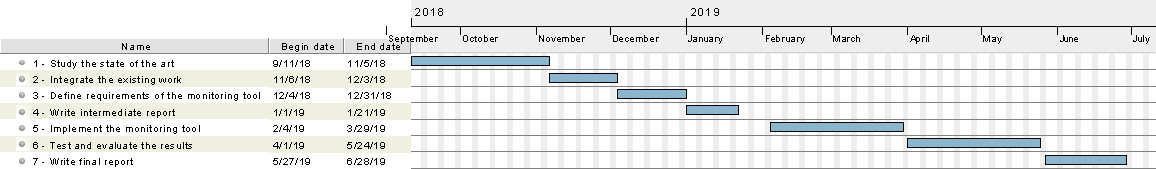
\includegraphics[height=0.234\textwidth]{images/proposed_work_plan_semester_1_and_2.pdf}
        \caption{Proposed work plan for first and second semesters.}
        \label{fig:proposed_work_plan_semester_1_and_2}
        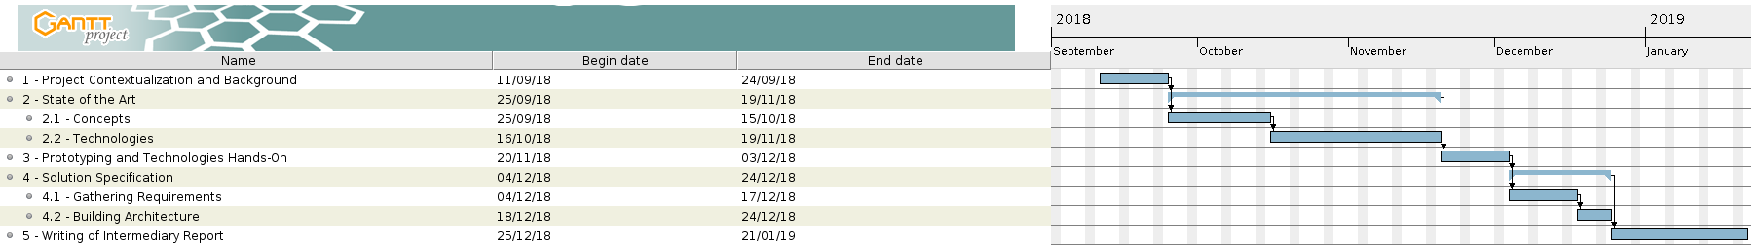
\includegraphics[height=0.3\textwidth]{images/real_work_plan_semester_1.pdf}
        \caption{Real work plan for first semester.}
        \label{fig:real_work_plan_semester_1}
    \end{figure}
\end{landscape}

\begin{landscape}
    \begin{figure}
        %\includegraphics[width=1.0\textwidth]{Image.eps}
        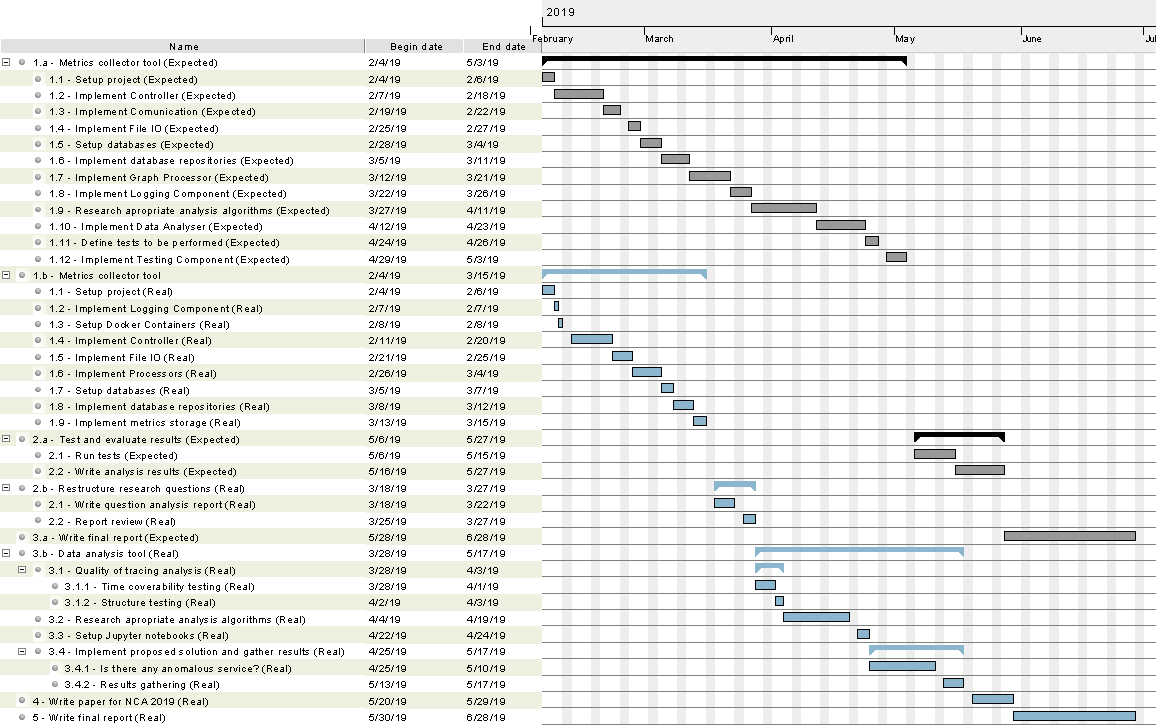
\includegraphics[height=1.0\textheight]{images/complete_work_plan_semester_2.pdf}
        \caption{Real and expected work plans for second semester.}
        \label{fig:complete_work_plan_semester_2}
    \end{figure}
\end{landscape}

\checkoddpage
\ifthenelse{\boolean{oddpage}}
{ % Odd page
    \newpage
    \blankpage}
{ % Even page
}
\glsresetall
\chapter{State of the Art}
\label{chap:state_of_the_art}

In this Chapter, we discuss the core concepts regarding the project, the most modern technology for the purpose today and related work in the area. All the information presented results from work of research through published articles, knowledge exchange and web searching.

First, the main purpose of Section~\ref{sec:concepts}~-~\nameref{sec:concepts} is to introduce and provide a brief explanation about the core concepts to the reader. Second, Section~\ref{sec:technologies}~-~\nameref{sec:technologies}, all the relevant technologies are analysed and discussed. In the final Section~\ref{sec:related_work}~-~\nameref{sec:related_work}, published articles and posts of related work are presented and possible research directions are discussed.

\section{Concepts}
\label{sec:concepts}

The following concepts represents the baseline to understand the work related to this research project. First an explanation of higher level of concepts that composes the title of this thesis are presented in Subsections~\ref{subsec:microservices} and~\ref{subsec:observability_and_controlling_performance}. The following Subsections~\ref{subsec:distributed_tracing} to~\ref{subsec:time_series}, aim to cover topics  related to previous concepts:~\nameref{subsec:distributed_tracing}, ~\nameref{subsec:graphs} and~~\nameref{subsec:time_series}.

\subsection{Microservices}
\label{subsec:microservices}

The term ``micro web services'' was first used by Dr. Peter Rogers during a conference on cloud computing in 2005, and evolved later on to ``Microservices'' at an event for software architects in 2011, where the term was used to describe a style of architecture that many attendees were experimenting with at the time. Netflix and Amazon were among the early pioneers of microservices~\cite{MauersbergerMicroservices}.

Microservices is ``an architectural style that structures an application as a collection of loosely coupled services, which implement business capabilities''~\cite{Dragoni2017, microservices_definition}.

This style of software development has a very long history and has being introduced and evolving due to software engineering achievements in the later years regarding cloud distributed computing infrastructures, \gls{api} improvements, agile development methodologies and the emergence of the recent phenomenon of containerized applications. ``A container is a standard unit of software that packages up code and all its dependencies so the application runs quickly and reliably from one computing environment to another, communicating with others through an \gls{api}''~\cite{Pahl2017}.

In Microservices, services are small, specifically calibrated to perform a single function, also each service is designed to be autonomous, resilient, minimal and composable. This framework brings a culture of rapid iteration, automation, testing, and continuous deployment, enabling teams to create products and deploy code exponentially faster than ever before~\cite{Newman}.

%The core concept of microservices stands in isolation, or by other words, what everyone wants to achieve when building a software with microservices in mind, is to share less things between the services and deal with correlated failures. In this sense, a service is a small part of the entire system (e.g. Get messages microservice), and represents a tiny feature of the whole service (e.g. Chat Service). To do this, normally every microservice is encapsulated inside a container (e.g. Docker container~\cite{docker}), and each runs in its own process and communicates with the other using lightweight mechanisms, often an \gls{http} resource \gls{api}. 

Until the rising of Microservices based architecture, the Monolithic architectural style was the most used. This style has a the particularity of produce software composed all in one piece. All features are bundled, packaged and deployed in a single tier application using a single code base.

Figure~\ref{fig:monolithic_and_microservices} aims to give a comparison between both architectural styles, Monolithic and Microservices, and provide an insight about the differences between them.

\begin{figure}[H]
    \centering
    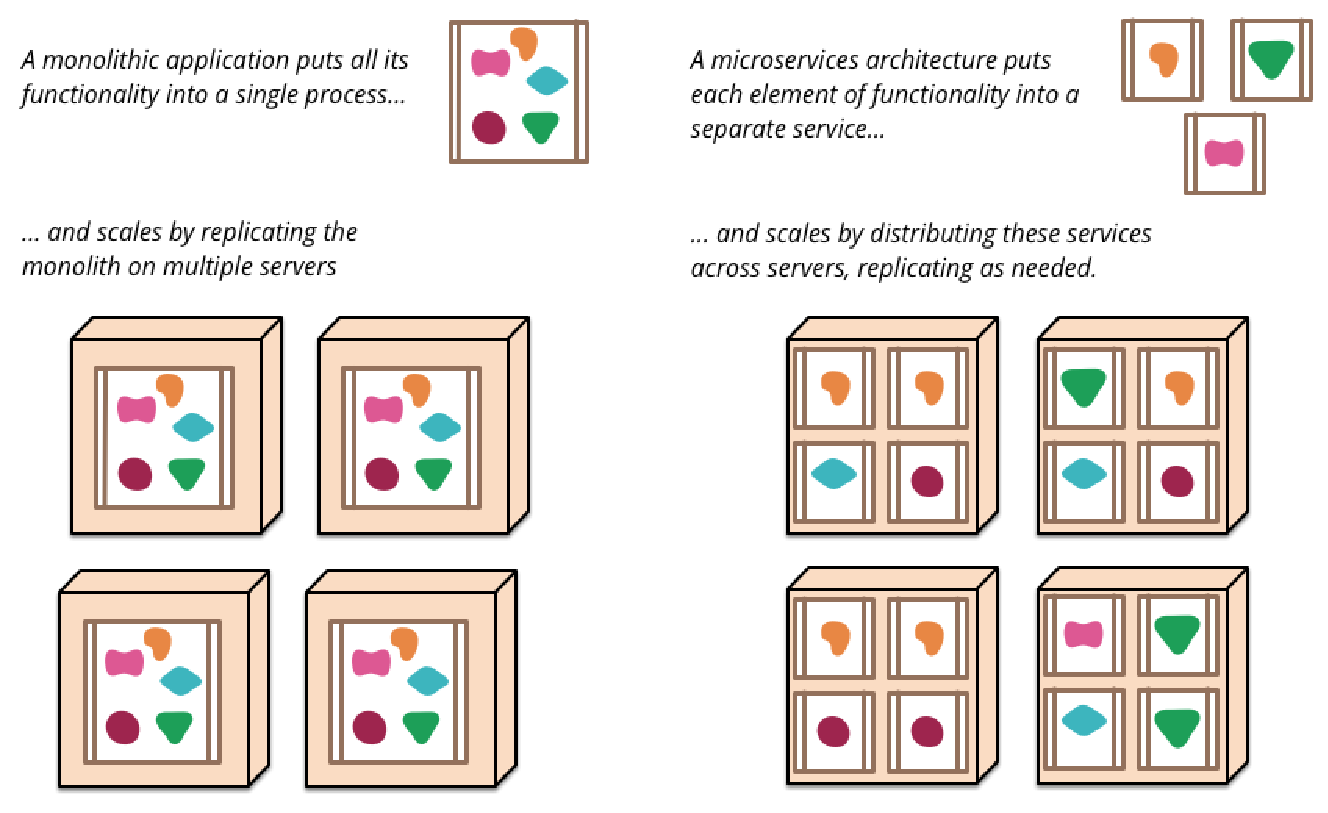
\includegraphics[width=1.00\textwidth]{monolithic_and_microservices.pdf}
    \caption{Monolithic and Microservices architectural styles~\cite{microservices}.}
    \label{fig:monolithic_and_microservices}
\end{figure}

Both styles presented have their own advantages and disadvantages. To briefly present some of them, two examples are provided, one for each architectural style. First example: if one team needs to develop a single process system, e.g., e-Commerce application, that authorizes customer, takes an order, check products inventory, authorize payment and ships ordered products. The best alternative is to use Monolithic architecture, because they can develop every feature in a single software package due to the application simplicity, however, if the client starts to demand hard changes and additional features in the solution, the code base may tend to increase into ``out of control'', leading to more challenging and time consuming changes. Second example, if one team needs to develop a complex and huge service that needs to scale, e.g., Video streaming service, the best alternative is to use Microservices architecture, because they can tackle the problem of complexity by decomposing the application into a set of manageable small services which are much faster to develop and test by individual organized teams, and thus, it will be easier to maintain the code base due to decoupling, however, it will be harder to monitor and manage the entire platform due to additional complexity associated with distributed systems.

Taking into consideration this increasing difficulty in monitoring and managing large Microservice based platforms, one must be aware and observe system behaviour to be able to control it. Therefore, in the next Subsection~\ref{subsec:observability_and_controlling_performance}, the core concept of~\nameref{subsec:observability_and_controlling_performance} is explained.

\subsection{Observability and Controlling Performance}
\label{subsec:observability_and_controlling_performance}

This Subsection aims to provide an introduction to some theory concepts about Observability and Performance Controlling, regarding distributed software systems.

Observability is a meaningfully extension of the word observing. Observing is ``to be or become aware of, especially through careful and directed attention; to notice'~'\cite{observing_definition}. The term Observability comes from the world of engineering and control theory. Observability is not a new term in the industry, however it has gain more focus in the last years due to \gls{devops} raising. It means by definition ``to measure of how well internal states of a system can be inferred from knowledge of its external outputs''~\cite{observability}. Therefore, if our good old software systems and applications do not adequately externalize their state, then even the best monitoring can fall short.

Controlling in control systems is ``to manage the behaviour of a certain system''~\cite{control_systems}. Controlling and Observability are dual aspects of the same problem~\cite{observability}, as we need to have information to infer state and be able take action. E.g., When observing an exponential increase in the \gls{cpu} load, the system scales horizontally invoking more machines and spreading the work between them to easy handle the work. This is a clear and simple example that conjugates the terms presented, we have: values that are observed ``Observability'' and action that leads to system control ``Controlling Performance''.

When we want to understand the working and behaviour of a system, we need to watch it very closely and pay special attention to all details and information it provides. Microservice based systems produce multiple types of information if instrumented. These type of information are the ones mentioned in Chapter~\ref{chap:introduction}: Monitoring, Tracing and Logging. In this thesis, the goal is to use tracing data thus, this type of produced information is the one to focus.

In the next Subsection~\ref{subsec:distributed_tracing}~-~\nameref{subsec:distributed_tracing}, the type of data mentioned before is presented and explained in detail.

\subsection{Distributed Tracing}
\label{subsec:distributed_tracing}

%\todo{How to introduce Google Dapper~\cite{Sigelman2010}}

Distributed tracing~\cite{Sambasivan2016a} is a method that comes from traditional tracing, but in this case acts in a distributed system at the work-flow level. It is used to profile and monitor applications, especially those built using microservice architectures and, in the end, it can be used to help DevOps teams pinpoint where failures occur and what causes system problems.

From this concept, standards emerged, like the best-known OpenTracing~\cite{open_tracing_data_model_specification}. The OpenTracing standard, follows the model proposed by Fonseca~\textit{et al.}~\cite{fonseca2007x}, which defines traces as a tree of spans, which represent scopes or units of work (i.e., thread, function, service) and follows their executing through the system.

OpenTracing uses dynamic, fixed-width metadata to propagate causality between spans, meaning that each span has a \emph{TraceID} common to all spans of that trace, as well as a \emph{SpanID} and \emph{ParentID} that are used to represent parent/child relationships between them~\cite{sambasivan2014so}.

The standard defines the format for spans and the semantic~\cite{open_tracing_semantic_specification, open_tracing_semantic_conventions} conventions for their content / annotations.

%Usually, the span has an operation name, the start time of the operation, its duration and some annotations regarding the operation itself. An example of a span can be an HTTP call or a Remote Procedure Call (RPC). 

Figure~\ref{fig:sample_trace_over_time} provides a clear insight about how spans are related to time and with each other.

\begin{figure}[H]
    \centerline{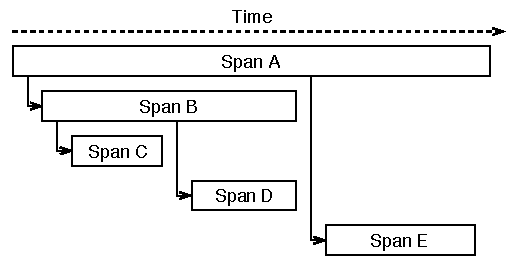
\includegraphics[width=1.0\linewidth]{images/trace.pdf}}
    \caption{Sample trace over time.}
    \label{fig:sample_trace_over_time}
\end{figure}

In Figure~\ref{fig:sample_trace_over_time} there are a group of five spans spread through time that represents a trace. A trace is a group of spans that share the same \emph{TraceID}.  A trace is a representation of a data/execution path in the system. A span represents the logical unit of work in the system. A trace can also be a span, if there is only one span presented in the trace. One span can cause another.

Causality relationship between spans can be observed in Figure~\ref{fig:sample_trace_over_time}, where ``Span A'' causes ``Span B'' and ``Span E'', moreover, ``Span B'' causes ``Span C'' and ``Span D''. From this we say that ``Span A'' is parent of ``Span B'' and ``Span E''. Likewise, ``Span B'' and ``Span E'' are children of ``Span A''. In this case, ``Span A'' does not have a parent, it is an ``orphan span'' and therefore, is the root span and the origin of this whole trace. Spans carry with them metadata like e.g., \emph{SpanID} and \emph{ParentID}, that allows to infer this relationships.

Disposition of spans over time is another clear fact that can be observed from the representation in Figure~\ref{fig:sample_trace_over_time}. Spans have a begin and an end in time. This causes them to have a duration. Spans are spread through time, however they usually stay inside parent boundaries, this means that the duration of a parent span always covers durations of their children. Considering a parent and a child spans, if they are related, the parent span always start before child span, also, the parent span always end after child span. Note that nothing prevents multiple spans to start in the same exact moment. Span also carry with them metadata like e.g., \emph{Timestamp} and \emph{Duration}, that allows to infer their position in time and when they end.

An example of a span can be an \gls{http} call or a \gls{rpc} call. We may think of the following cases to define each operation inherent to each box presented in Figure~\ref{fig:sample_trace_over_time}: A - ``Get user info'', B - ``Fetch user data from database'', C - ``Connect to MySQL server'', D - ``Can't connect to MySQL server'' and E - ``Send error result to client''.

In the data model specification, the creators of OpenTracing say that: ``with a couple of spans, we might be able to generate a span tree and model a directed graph of a portion of the system''~\cite{open_tracing_data_model_specification}. This is due to the causal relationships they represent. Figure~\ref{fig:span_tree_example} provides an example of a span tree.

\begin{figure}[H]
    \centering
    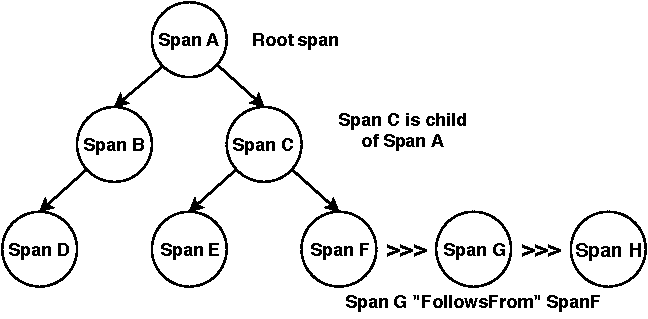
\includegraphics[width=1.0\linewidth]{span_tree_example.pdf}
    \caption{Span Tree example.}
    \label{fig:span_tree_example}
\end{figure}

Figure~\ref{fig:span_tree_example} contains a span tree representation with a trace containing eight spans. As said before,every span must be a child of some other span, unless it is the root span, this is very clear in a span tree visualization with the usage of the root node. With this causal relationship, a path through the system can be retrieved. For example, if for example every span processes in a different endpoint represented by letters presented in the span tree, one may generate the request path: A ---$>$ B ---$>$ D. This means that our hypothetical request passed through machine A, B and D, or if it were services, the request passed from service A, to B and finally to D. From this, we can generate the dependency graph of the system (explained in the Subsection~\ref{subsec:graphs}~-~\nameref{subsec:graphs}).

This type of data is extracted as trace files or streamed over transfer protocols like e.g., \gls{http}, from technologies like Kubernetes~\cite{what_is_kubernetes}, OpenStack~\cite{what_is_opensatck}, and other cloud or distributed management system technologies that implements some kind of system or code instrumentation using, for example, OpenTracing~\cite{what_is_opentracing} or OpenCensus~\cite{what_is_opencensus}. Tracing contains some vital system details as they are the result of system instrumentation and therefore, this data can be used as a resource to provide observability over the distributed system.

As said before, from the causality relationship between spans we can generate a dependency graph of the system. The next Subsection~\ref{subsec:graphs}~-~\nameref{subsec:graphs} aims to provide a clear understand of this concept and how they relate with distributed tracing.

\subsection{Graphs}
\label{subsec:graphs}

From distributed tracing we can be able to extract the system dependency graph from a representative set of traces. To introduce the concept of Graph, ``A Graph is a set of vertices and a collection of directed edges that each connects an ordered pair of vertices''~\cite{graph_standard_definition}.

Taking the very common sense of the term and to provide notation, a graph, $G$, is an ordered pair $G = (V, E)$, where $V$ are the vertices/nodes and $E$ are the edges.

Graphs are defined by:

\begin{itemize}
    \item Node: Are the entities in the graph. They can hold any number of attributes (key-value pairs) called properties. Nodes can be tagged with labels, representing their different roles in a domain. Node labels may also serve to attach metadata (such as index or constraint information) to certain nodes;
    \item Edge (or Relationships): provide directed, named, semantically-relevant connections between two node entities;
    \item Property: can be any kind of metadata attached to a certain Node or a certain Edge.
\end{itemize}

Also, there are multiple types of graphs, they can be:

\begin{enumerate}
    \item Undirected-Graph: the set of edges without orientation between a pair of nodes;
    \item Directed-Graph: the set of edges have one and only one direction between a pair of nodes;
    \item Multi-Directed-Graph: multiple edges have more than one connection between a pair of nodes that represents the same relationship.
\end{enumerate}

Figure~\ref{fig:graphs_types} gives us a simple visual representation of what a graph really is for a more clear understanding.

\begin{figure}[H]
    \centering
    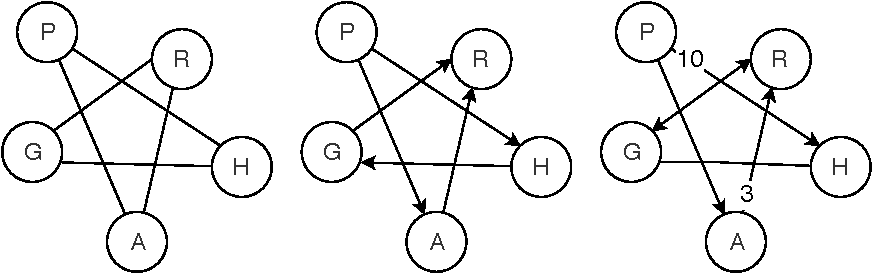
\includegraphics[width=1.00\textwidth]{images/graph_representations.pdf}
    \caption{Graphs types.}
    \label{fig:graphs_types}
\end{figure}

In Figure~\ref{fig:graphs_types} three identical graphs are presented and each one is composed by five nodes, however, they are not equal because each one has it own type. They belong respectively to each type enumerated above. From left to right, the first graph is a Undirected-Graph, the second one is a Directed-Graph and the last one is a Multi-Directed-Graph.

The last graph has some numbers in some edges. Every graph can have this annotations. These can provide some information about the connection between the pair of nodes. For example, in distributed systems context, if this graph represents our system dependency graph, and nodes $H$ and $P$ hypothetical services, the edge between them could represent calls between these two service and the notation number the number of calls with respect to the edge direction. Therefore, in this case, we would have 10 requests from incoming from $P$ to $H$.

Figure~\ref{fig:service_dependency_graph} provides a clear insight about service dependency graphs.

\begin{figure}[H]
    \centering
    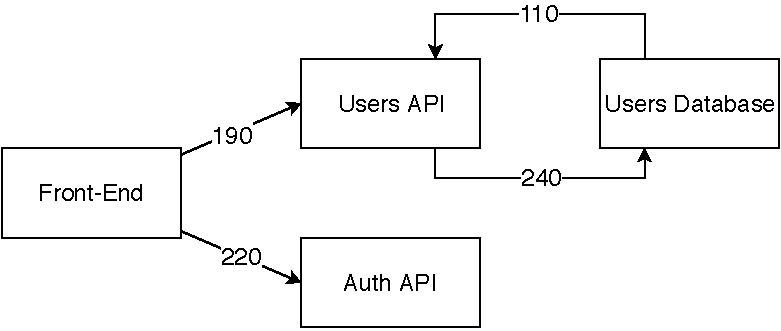
\includegraphics[width=1.00\textwidth]{images/graph_service_representation.pdf}
    \caption{Service dependency graph.}
    \label{fig:service_dependency_graph}
\end{figure}

In Figure~\ref{fig:service_dependency_graph}, a representation of a service dependency graph is provided. Service dependency graphs are graphs of type Multi-Directed-Graph, because they have multiple edges with more than one direction between a pair of services(Nodes). In this representation, there are multiple services involved, each inside a box. The edges between boxes (Nodes), indicate the number of calls that each pair of services invoked, e.g., ``Users API'' called ``Ùsers Database'' 240 times. These dependency graphs gives the state of the system in a given time interval. This can be useful to study the changes in the morphology of the system, e.g., a service disappeared and a set of new ones appeared. Other interesting study could be the variation in the amount of call between services.

Graphs are a way to model and extract information from tracing data. Another interesting approach could be to extract metrics in time from tracing because traces and spans are spread in time, and they have information about the state of the system at a given instant. The next Subsection~\ref{subsec:time_series}~-~\nameref{subsec:time_series} provides an introduction to a data representation model.

\subsection{Time Series}
\label{subsec:time_series}

Time-Series are a way of representing data as a time-indexed series of values. This kind of data is often arise when monitoring systems, industrial processes, tracking corporate business metrics or sensor measurements. Figure~\ref{fig:time_series_example} provides a visual example of this way of data representation.

\begin{figure}[H]
    \centering
    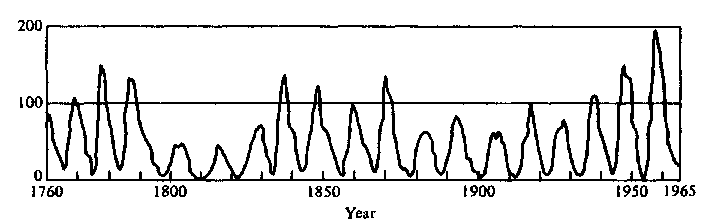
\includegraphics[width=1.00\textwidth]{images/time_series_example.pdf}
    \caption{Time series: Annual mean sunspot numbers for 1760-1965~\cite{Brillinger2006}.}
    \label{fig:time_series_example}
\end{figure}

In Figure~\ref{fig:time_series_example}, Brillinger \textit{D.}~\cite{Brillinger2006} presents a visual representation of a time-series as a collection of values in time. These values are measurements of sunspot means gathered from 1960-1965. In this case, measurements come from natural origin, however, one can perform observations of e.g., \gls{cpu} load, system uptime / downtime and network latency.

As these processes are not random, autocorrelation can be exploited to extract insight from the data, such as predict patterns or detect anomalies. Therefore, time-series data can be analysed to detect anomalies present in the system. One way to do this is to look for outliers~\cite{Liu2004} in the multidimensional feature set. Anomaly detection in time series data is a data mining process used to determine types of anomalies found in a data set and to determine details about their occurrences. Anomaly detection methods are particularly interesting for our data set since it would be impossible to manually tag the set of interesting anomalous points. Figure~\ref{fig:time_series_anomaly_detection_example} provides a simple visual representation of anomaly detection in time series data.

\begin{figure}[H]
    \centering
    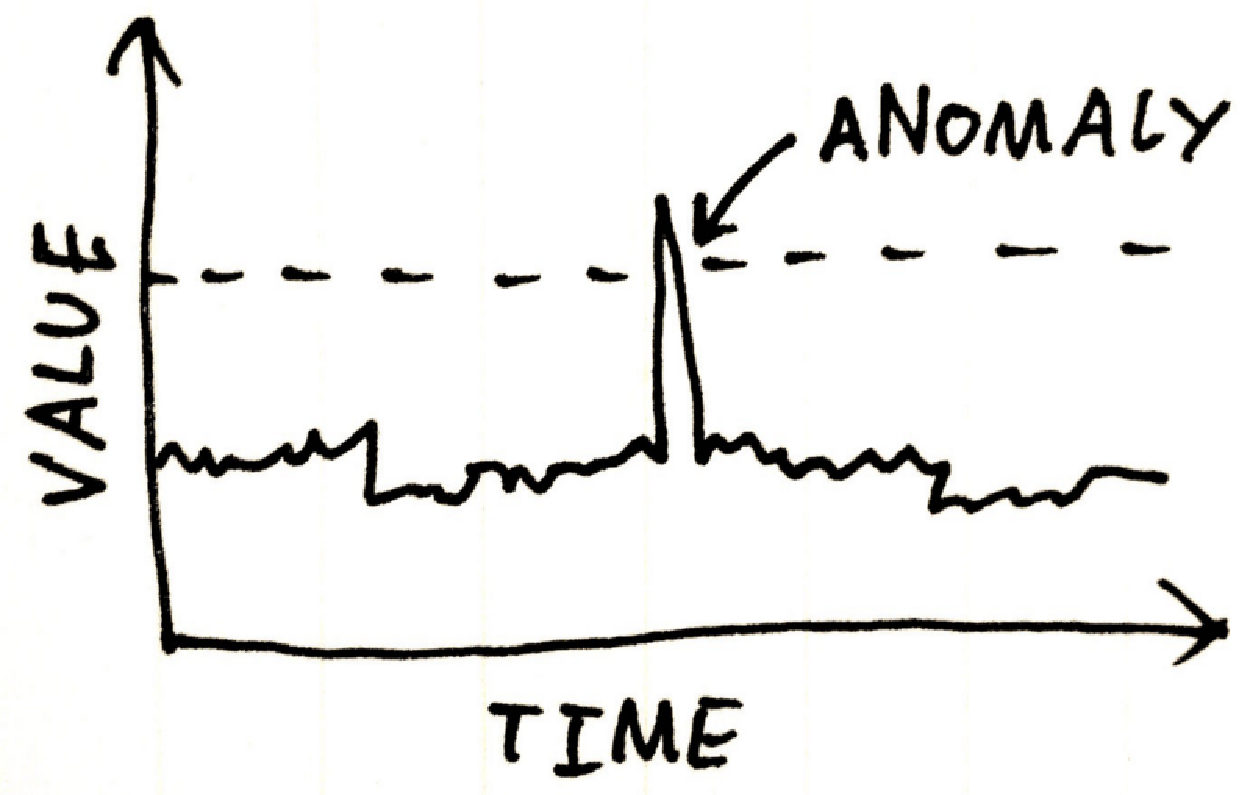
\includegraphics[width=0.50\textwidth]{images/time_series_anomaly_detection_example.pdf}
    \caption{Anomaly detection in Time Series~\cite{NikolajBomannMertz}.}
    \label{fig:time_series_anomaly_detection_example}
\end{figure}

In Figure~\ref{fig:time_series_anomaly_detection_example}, there is a clear spike in values from this time series measurements. This can be declared an outlier because it is a strange value considering the range of remaining measurements and therefore, it is considered an anomaly. In this example, anomaly detection is easy to perform by a Human, however, in mostly cases nowadays, due to great variation of values and plethora of information that can be gathered, perform this detection manually is impracticable, thus automatic anomaly detection using Machine Learning techniques are used nowadays.

Anomaly detection in time series data is a data mining process used to determine types of anomalies found in a data set and to determine details about their occurrences. This auto anomaly detection method has lots of usage due to the impossible work of tag manually the interesting set of anomalous points. Auto anomaly detection has a wide range of applications such as fraud detection, system health monitoring, fault detection, event detection systems in sensor networks, and so on.

After explaining the core concepts, foundations for the work presented in this thesis, to the reader, technologies capable of handling this types of information are presented and discussed in next Section~\ref{sec:technologies}~-~\nameref{sec:technologies}.

\section{Technologies}
\label{sec:technologies}

In this section are presented technologies and tools capable of handling the types of information discussed in the previous Section~\ref{sec:concepts}~-~\nameref{sec:concepts}.

The main tools covered are:~\ref{subsec:distributed_tracing_tools}~-~\nameref{subsec:distributed_tracing_tools}, for distributed tracing data handling, \ref{subsec:graph_manipulation_and_processing_tools}~-~\nameref{subsec:graph_manipulation_and_processing_tools} and~\ref{subsec:graph_database_tools}~-~\nameref{subsec:graph_database_tools}, for graph processing and storage, and~\ref{subsec:time_series_database_tools}~-~\nameref{subsec:time_series_database_tools}, for time series value storage.

\subsection{Distributed Tracing Tools}
\label{subsec:distributed_tracing_tools}

This Subsection presents the most used and known distributed tracing tools. These tools are mainly oriented for tracing distributed systems like microservices-based applications. What they do is to fetch or receive trace data from this kind of complex systems, treat the information, and then present it to the user using charts and diagrams in order to explore the data in a more human-readable way. One of the best features presented in this tools, is the possibility to perform queries on the tracing (e.g., by trace id and by time-frame). Table~\ref{table:distributed_tracing_tools} presents the most well-known open source tracing tools.

\begin{table}[]
    \caption{Distributed tracing tools comparison.}
    \label{table:distributed_tracing_tools}
    \centering
    \begin{tabularx}{\linewidth} {
            >{\hsize=0.70\hsize}X|
            >{\hsize=1.15\hsize}X|
            >{\hsize=1.15\hsize}X|}
        \cline{2-3}

         & Jaeger~\cite{jaeger_github}
         & Zipkin~\cite{zipkin_github}                                                                                                                                                                                  \\ \hline \hline
        \multicolumn{1}{|l|}{\textbf{Brief description}}
         & Released as open source by Uber Technologies and is used for monitoring and troubleshooting microservices-based distributed systems. Was inspired by Zipkin.
         & Helps gather timing data needed to troubleshoot latency problems in microservice architectures and manages both the collection and lookup of this data. Zipkin's design is based on the Google Dapper paper. \\ \hline
        \multicolumn{1}{|l|}{\textbf{Pros}}
         & OpenSource; \newline
        Docker-ready; \newline
        Collector interface is compatible with Zipkin protocol; \newline
        Dynamic sampling rate; \newline
        Browser UI.
         & OpenSource; \newline
        Docker-ready; \newline
        Allows lots of span transport ways (HTTP, Kafka, Scribe, AMQP); \newline
        Browser UI.                                                                                                                                                                                                     \\ \hline
        \multicolumn{1}{|l|}{\textbf{Cons}}
         & Only supports two span transport ways (Thrift and HTTP).
         & Fixed sampling rate.                                                                                                                                                                                         \\ \hline
        \multicolumn{1}{|l|}{\textbf{Analysis}}
         & Dependency graph view; \newline
        Trace comparison (End 2018).
         & Dependency graph view.                                                                                                                                                                                       \\ \hline
        \multicolumn{1}{|l|}{\textbf{Used by}}
         & Red Hat; \newline
        Symantec; \newline
        Uber. \newline
         & AirBnb; \newline
        IBM; \newline
        Lightstep.                                                                                                                                                                                                      \\ \hline
    \end{tabularx}
\end{table}

In Table~\ref{table:distributed_tracing_tools}, we can see that these two tools are very similar. Both are open source projects, allow docker containerization and provide a browser ui to simplify user interaction. Jaeger was created by Uber and the design was based on Zipkin, however, it does not provide much more features. The best feature that was released for Jaeger in the past year was the capability of perform trace comparison, where the user can select a pair of traces and compare them in terms of structure. This is a good effort in additional features, but it is short in versatility because we can only compare a pair of traces in a ``sea'' of thousands, or even millions.

These tools aim to collect trace information and provide a user interface with some query capabilities for \gls{devops} to use. However they are always focused on span and trace lookup and presentation, and do not provide a more interesting analysis of the system, for example to determine if there is any problem related to some microservice presented in the system. This kind of work falls into the user, \gls{devops}, as they need to perform the tedious work of investigation and analyse the tracing with the objective of find anything wrong with them.

This kind of tools can be a good starting point for the problem that we face, because they already do some work for us like grouping the data generated by the system and provide a good representation for them.

In next Subsection~\ref{subsec:graph_manipulation_and_processing_tools}, graph manipulation and processing tools are presented and discussed.

\subsection{Graph Manipulation and Processing Tools}
\label{subsec:graph_manipulation_and_processing_tools}

Distributed tracing is a type of data produced by Microservice based architectures. This type of data is composed by traces and spans. With a set of related spans, a service dependency graph can be produced. This dependency graph is a Multi-Directed-Graph, as presented in Subsection~\ref{subsec:graphs}. Therefore, with this data at our disposal, there is the need of a graph manipulation and processing tool.

In this Subsection, the state of the art about graph manipulation and processing tools is presented. Graphs are non-linear data structure representations consisting of nodes and edges. Nodes are sometimes also referred to as vertices and edges are lines or arcs that connect any pair of nodes in the graph. This data structure takes some particular approaches when handling their contents, because there are some special attributes related. For example, perform the calculation of the degree of some node -- degree of a node is the number of edges that connect to the node itself; Calculate how many nodes entered and exited the graph by comparing it to another one; Know the difference in edges between two distinct graphs~\cite{Trudeau1993}.

Taking into consideration this data structure, the particularities involved and the need to use graphs to manipulate service dependencies, frameworks with features capable of handling and retrieving graphs are a need. Therefore, Table~\ref{table:graph_manipulation_and_processing_tools_comparison} presents a comparison of the main tools available at the time for graph manipulation and processing.

\begin{table}[H]
    \caption{Graph manipulation and processing tools comparison.}
    \label{table:graph_manipulation_and_processing_tools_comparison}
    \centering
    \begin{tabularx}{\linewidth} {
            >{\hsize=0.3\hsize}X|
            >{\hsize=1.0\hsize}X|
            >{\hsize=1.0\hsize}X|
            >{\hsize=1.0\hsize}X|}
        \cline{2-4}

         & Apache Giraph \cite{apache_giraph}
         & Ligra \cite{ligra_graph_processing_framework}
         & NetworkX \cite{networkx}                                                                                                                                                       \\ \hline \hline
        \multicolumn{1}{|l|}{\textbf{Description}}
         & An iterative graph processing system built for high scalability. Currently used at Facebook to analyse the social graph formed by users and their relationships.
         & A library collection for graph creation, analysis and manipulation of networks.
         & A Python package for the creation, manipulation, and study of structure, dynamics, and functions of complex networks.                                                          \\ \hline
        \multicolumn{1}{|l|}{\textbf{Licence}~\cite{Morin2012}}
         & Free Apache 2.
         & MIT.
         & BSD - New License.                                                                                                                                                             \\ \hline
        \multicolumn{1}{|p{2cm}|}{\textbf{Supported languages}}
         & Java and Scala.
         & C and C++.
         & Python.                                                                                                                                                                        \\ \hline
        \multicolumn{1}{|l|}{\textbf{Pros}}
         & Distributed and very scalable; \newline
        Excellent performance -- Process one trillion edges using 200 modest machines in 4 minutes.
         & Handles very large graphs; \newline
        Exploit large memory and multi-core \gls{cpu} -- Vertically scalable.
         & Good support and very easy to install with Python; \newline
        Lots of graph algorithms already implemented and tested. \newline                                                                                                                 \\ \hline
        \multicolumn{1}{|l|}{\textbf{Cons}}
         & Uses ``Think-Like-a-Vertex'' programming model that often forces into using sub-optimal algorithms, thus is quite limited and sacrifices performance for scaling out; \newline
        Unable to perform many complex graph analysis tasks because it primarily supports Bulk synchronous parallel.
         & Lack of documentation and therefore, very hard to use; \newline
        Does not have many usage in the community.
         & Not scalable (single-machine); \newline
        High learning curve due to the maturity of the project; \newline
        Begins to slow down when processing high amount of data -- 400.000+ nodes.                                                                                                        \\ \hline
    \end{tabularx}
\end{table}

Table~\ref{table:graph_manipulation_and_processing_tools_comparison} presents some key points to consider when choosing a graph manipulation and processing tool.

First, one aspect to be considered when comparing them is the scalability and performance that each provide. Apache Giraph is the best tool in this field, since it is implemented with distributed and parallel computation, which allows it to scale to multiple-machines, sharing the load between them, and processing data large quantities of data in less time than the remaining presented tools. On the opposite side, NetworkX, only works in a single-machine environment which does not allow it scale to multiple-machines. Ligra, like the previous tool, works in a single-machine environment, however it benefits from vertical scale on a single-machine, which allows to exploit multi-core \gls{cpu} and large memory. NetworkX and Ligra are tools that can present a bottleneck in a system where the main focus is to handle large amounts of data in short times.

\,

Secondly, another aspect to be considered is the support and quantity of implemented graph algorithms available on the frameworks. NetworkX have advantages in this aspect, because it contains implementation of the majority graph algorithms defined and studied in graph and networking theory. Also, due to project maturity, it has a good documentation support from the community who keeps all the information updated. Ligra framework has lack of documentation, which causes tremendous difficulty for developers to use and know what are the implemented features. Apache Giraph, does not support a large set of graph processing algorithms due to implementation constraints.

Figure~\ref{fig:graph_tools_comparison} gives a clear insight when comparing these tools from two features -- scalability / performance against implementation of graph algorithms.

\begin{figure}[H]
    \centering
    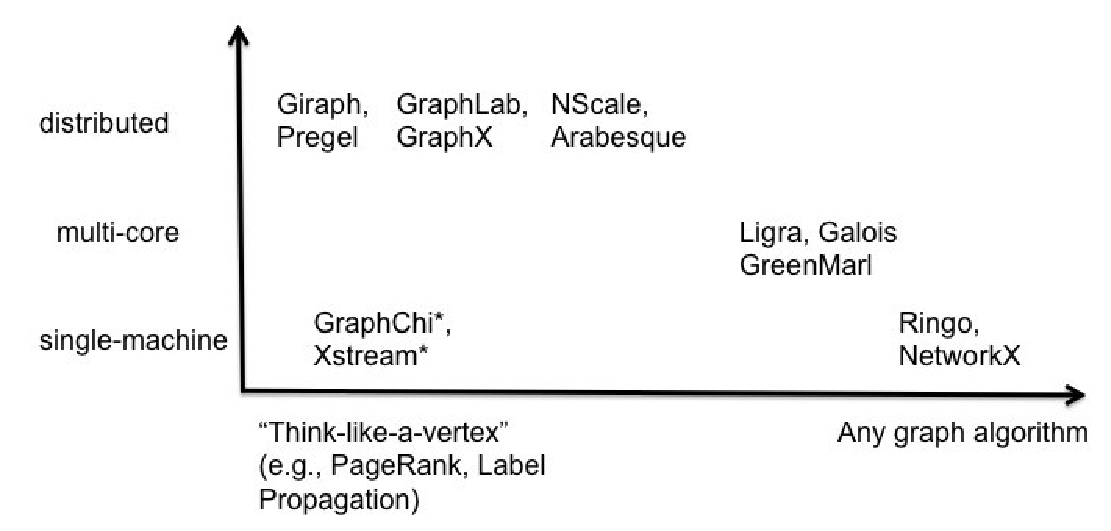
\includegraphics[width=1.0\linewidth]{images/graph_manipulation_tools_diagram_comparison.pdf}
    \caption{Graph tools: Scalability vs. Algorithm implementation~\cite{graph_data_management_systems}.}
    \label{fig:graph_tools_comparison}
\end{figure}

In Figure~\ref{fig:graph_tools_comparison} we can observe tools disposition regarding the two aspect key points explained before. This figure contains all tools presented over two featured axis: one for scalability and the other for implementation of graph algorithms. Tools placement in this chart proves and reinforces the comparison presented before. Apache Giraph and NetworkX are placed in the edges of these features, which means that Apache Giraph can be found in the upper left region of the chart -- highly distributed but minimally in graph algorithms implementation --, and NetworkX is in the lower right region -- minimally distributed but highly in graph algorithms implementation.

After discussing tools capable of manipulate and process graphs, their storage is a need for later usage. \gls{gdb} storage technologies are presented in next Subsection~\ref{subsec:graph_database_tools}~-~\nameref{subsec:graph_database_tools}.

\subsection{Graph Database Tools}
\label{subsec:graph_database_tools}

Graph databases represent a way of persisting graph information. After having instantiated a Graph, processed it in volatile memory, they can be stored in persistent memory for later use. To do this one can use a \gls{gdb}. A \gls{gdb} is ``a database that allows graph data storing and uses graph structures for semantic queries with nodes, edges and properties to represent them''~\cite{Celko2013}.

\,

Based upon the concept of a mathematical graph, a graph database contains a collection of nodes and edges. A node represents an object, and an edge represents the connection or relationship between two objects. Each node in a graph database is identified by a unique identifier that expresses key value pairs. Additionally, each edge is defined by a unique identifier that details a starting or ending node, along with a set of properties. Graph databases are becoming popular due to Machine Learning and Artificial Intelligence grows, since a number of Machine Learning algorithms are inherently graph algorithms~\cite{FavioVazquez2019}.

Furthermore, in this research service dependency graphs are highly used, thus the need to use a \gls{gdb}. Table~\ref{table:graph_databases_comparison} contains the most well-known \gls{gdb}.

\begin{table}[H]
    \caption{Graph databases comparison.}
    \label{table:graph_databases_comparison}
    \centering
    \begin{tabularx}{\linewidth} {
            >{\hsize=0.3\hsize}X|
            >{\hsize=1.0\hsize}X|
            >{\hsize=1.0\hsize}X|
            >{\hsize=1.0\hsize}X|}
        \cline{2-4}

         & ArangoDB \cite{arangodb_documentation}
         & Facebook TAO \cite{facebook_tao_article}
         & Neo4J \cite{neo4j_documentation}                                                                                               \\ \hline \hline
        \multicolumn{1}{|l|}{\textbf{Description}}
         & A NoSQL database that uses a proper query language to access the database.
         & TAO, “The Associations and Objects”, is a proprietary graph database, developed by Facebook, used to store the social network.
         & The most popular open source graph database, completely open to the community.                                                 \\ \hline
        \multicolumn{1}{|l|}{\textbf{Licence}~\cite{Morin2012}}
         & Free Apache 2.
         & Proprietary.
         & GPLv3 CE.                                                                                                                      \\ \hline
        \multicolumn{1}{|p{2cm}|}{\textbf{Supported languages}}
         & C++; Go; Java; JavaScript; Python and Scala.
         & Go; Java; JavaScript; Python and Scala.
         & Java; JavaScript; Python and Scala.                                                                                            \\ \hline
        \multicolumn{1}{|l|}{\textbf{Pros}}
         & Multi data-type support (key/value, documents and graphs); \newline
        Allows combination of different data access patterns in a single query; \newline
        Supports cluster deployment.
         & Low latency $(~=100ms)$; \newline
        Accepts millions of calls per second; \newline
        Distributed database.
         & Supports ACID(Atomicity, Consistency, Isolation, Durability)~\cite{Sasaki2018}; \newline
        Most popular open source graph database.                                                                                          \\ \hline
        \multicolumn{1}{|l|}{\textbf{Cons}}
         & High learning curve due to AQL (Arango Query Language); \newline
        Has paid version with high price tag.
         & Not accessible to use.
         & Not able to scale horizontally.                                                                                                \\ \hline
    \end{tabularx}
\end{table}

From Table~\ref{table:graph_databases_comparison} we can notice that the state of the art for \gls{gdb} is not very pleasant, because the interest for this type of databases has began in the later years due to artificial intelligence and machine learning trends. Therefore, the offer presented in the field are limited.

Back in time, when social network tendency emerged, the development of this type of databases raised, and the most powerful technologies for graph storage where developed in closed source. One example is Facebook TAO database presented in Table~\ref{table:graph_databases_comparison}, a database developed by the company to support the entire social network, storing users in nodes and their relationships in edges. This database is described by having very low latency, which stands for high response time however, just a few scientific papers were found~\cite{facebook_tao_article,Amenya2018}.
%very few information regarding this tool can be found -- just some scientific papers

The remaining tools presented are available for usage. ArangoDB has multi data-type support, which means that a wider type of data structures are supported for storing in nodes and edges metadata. Also, it supports scalability through cluster deployment, however, this feature is only available in paid versions -- Arango SmartGraphs storage improves the writing of graph in distributed systems environment~\cite{arangodb_smart_graphs}. The biggest disadvantage of this database is the high learning curve associated with the usage of AQL (Arango Query Language), however, this disadvantage can be surpassed by using provided \gls{api} clients with the trade-off of loosing some control.

Neo4J is the most accepted \gls{gdb} by the open source community. This \gls{gdb}
has increased in popularity in the past years due to simplicity and easy support~\cite{Turu2017}. Trade-offs from this database consists in lack of support for scalability, which means that this database can only run on a single-machine environment, however, there are some users reporting that they were able to perform implementations and surpass the lack of support for horizontal scaling, but this is not tested~\cite{neo4j_scalable}.

Choosing a graph database can be hard because these tools are growing and the tendency for changes in features and tooling support is very high, however,  the decision falls on the question of easy of usage and horizontal scalability. This means that ArangoDB is a database more advised for big projects, where the size of graphs to store may surpass the limit of a single-machine, and Neo4J for simpler projects, where the focus are functionality testing and prototyping, and graph storage represents a side concern.

Next Subsection~\ref{subsec:time_series_database_tools}~-~\nameref{subsec:time_series_database_tools} covers the state of the art for tooling capable of storage values based in time.

\subsection{Time-Series Database Tools}
\label{subsec:time_series_database_tools}

In this Subsection, tools for storing time-indexed series of values are presented. This type of data is a need for this research due to the tight relation between distributed tracing and time, as explained in Subsections~\ref{subsec:distributed_tracing} and~\ref{subsec:time_series}. Also, service dependency graphs, as a representation of the system at a given time, can contain valuable information for monitoring Microservice systems. For this purpose, \gls{tsdb} are databases capable of storing time-series based values.

A \gls{tsdb} is ``A database optimised for time-stamped or time series data like arrays of numbers indexed by time (a date time or a date time range)''~\cite{Dunning2015}. These databases are natively implemented using specialised time-series theory algorithms to enhance their performance and efficiency, due to widely variance of access possible. The way this databases use to work on efficiency is to treat time as a discrete quantity rather than as a continuous mathematical dimension. Usually a \gls{tsdb} allows operations like create, enumerate, update, organise and destroy various time series entries in short access times.

This type of database is growing in usage and popularity because of Internet of Things (IoT) trend. Discussions in this area have increased over the past few years, and is expected that it keeps increasing, due to Ubiquitous Computing -- Raise of omnipresent and universal technologies. At the same time, \gls{tsdb} grows with this IoT tendency, because data mining from sensor spread geographically and sensors gather information through measurements in specific points in time. This information are usually stored in \gls{tsdb}~\cite{TanayPant2019}.

Table~\ref{table:time_series_databases_comparison} presents a comparison between two \gls{tsdb}: \textit{InfluxDb} and \textit{OpenTSDB}.

\begin{table}[H]
    \caption{Time-series databases comparison.}
    \label{table:time_series_databases_comparison}
    \centering
    \begin{tabularx}{\linewidth} {
            >{\hsize=0.70\hsize}X|
            >{\hsize=1.15\hsize}X|
            >{\hsize=1.15\hsize}X|}
        \cline{2-3}

         & InfluxDB \cite{influxdb}
         & OpenTSDB \cite{opentsdb}                                                                                                                                                                                                                                       \\ \hline \hline
        \multicolumn{1}{|l|}{\textbf{Description}}
         & An open-source time series database written in Go and optimised for fast, high-availability storage and retrieval of time series data in fields such as operations monitoring, application metrics, Internet of Things sensor data, and real-time analytics's.
         & A distributed and scalable \gls{tsdb} written on top of HBase; \newline
        OpenTSDB was written to address a common need: store, index and serve metrics collected from computer systems (network gear, operating systems and applications) at a large scale, therefore, making this data easily accessible and displayed.                   \\ \hline
        \multicolumn{1}{|l|}{\textbf{Licence}~\cite{Morin2012}}
         & MIT.
         & GPL.                                                                                                                                                                                                                                                           \\ \hline
        \multicolumn{1}{|p{2cm}|}{\textbf{Supported languages}}
         & Erlang, Go, Java, JavaScript, Lisp, Python, R and Scala.
         & Erlang, Go, Java, Python, R and Ruby.                                                                                                                                                                                                                          \\ \hline
        \multicolumn{1}{|l|}{\textbf{Pros}}
         & Scalable in the enterprise version; \newline
        Outstanding high performance; \newline
        Accepts data from \gls{http}, TCP, and UDP protocols; \newline
        SQL like query language; \newline
        Allows real-time analytics's.
         & Massively scalable; \newline
        Great for large amounts of time-based events or logs; \newline
        Accepts data from \gls{http} and TCP protocols; \newline
        Good platform for future analytical research into particular aggregations on event / log data; \newline
        Does not have paid version.                                                                                                                                                                                                                                       \\ \hline
        \multicolumn{1}{|l|}{\textbf{Cons}}
         & Enterprise high price tag; \newline
        Clustering support only available in the enterprise version.
         & Hard to set up; \newline
        Not a good choice for general-purpose application data.                                                                                                                                                                                                           \\ \hline
    \end{tabularx}
\end{table}

From Table~\ref{table:time_series_databases_comparison}, we can notice some similarities between these two \gls{tsdb} databases. Both \gls{tsdb} are capable scalable and accept \gls{http} and TCP transfer protocols for communication. InfluxDB and OpenTSDB are two open source time-series databases, however, the first one, InfluxDB, is not completely free, as it has an enterprise paid version, which is not very visible in the offer. This enterprise version offers, clustering support, high availability and scalability~\cite{influxdb_vs_opentsdb}, features that OpenTSDB offer for free. In terms of performance, InfluxDB surpasses and outperforms OpenTSDB in almost every benchmarks~\cite{Noor2017}. OpenTSDB has the benefits of being completely free and support the most relevant features, however it is very hard to set up and to develop for this database.

In the end, both \gls{tsdb} are bundled with good features, and the decision falls into how much performance is needed when choosing one. If the need is performance and access to the database in short amounts of time, with low latency responses, InfluxDB is the way to go, by other way, if there no restriction about the performance needed to query the database and money is a concern, the choice should be OpenTSDB.

Tooling for this project is presented. We have covered the most used technologies and core concepts in related to the field of tracing Microservices. Next Section~\ref{sec:related_work}~-~\nameref{sec:related_work}, will cover the related work performed in this area. Some ideas, approaches and developed solutions will be discussed.

\section{Related Work}
\label{sec:related_work}

This section aims to present the related work in the field of distributed tracing data handling and analysis. It is divided in three Subsections: first, \ref{subsec:mastering_aiops}~-~\nameref{subsec:mastering_aiops}, which covers a work carried out by Huawei, that uses machine learning -- deep learning -- methods to analyse data from distributed traces. Secondly, \ref{subsec:anomaly_detection_using_zipkin_tracing_data}~-~\nameref{subsec:anomaly_detection_using_zipkin_tracing_data}, a work of performed by Salesforce with the objective of analyse tracing from a distributed tracing tool. Finally, \ref{subsec:analysing_distributed_trace_data}~-~\nameref{subsec:analysing_distributed_trace_data}, a work by Pinterest, where the objective is to study latency in tracing data.

\subsection{Mastering AIOps}
\label{subsec:mastering_aiops}

Distributed tracing has only started to gain widespread acceptance in the industry recently, as a result of new architectural and software engineering practices, such as cloud-native, fine-grained systems and agile methodologies. Additionally, the increase in complexity resulting from the rise of web-scale distributed applications is a recent phenomenon. As a consequence of its novelty, there has been little research in the field so far.

A recent example, AIOps, an application of Artificial Intelligence to operations~\cite{rising_aiops} was introduced in $2016$~\cite{gartner_aiops}. This trend aims to use Artificial Intelligence for IT Operations in order to develop new methods to automate the enhance IT Operations. Driving this ``revolution'' are the following points:

\begin{itemize}
    \item First there is the additional difficulty of manually managing distributed infrastructures and system state;
    \item Secondly, the amount of data that has to be retained is increasing, creating a plethora of problems to the operators handling it;
    \item Third, the infrastructure itself is becoming more distributed across geography and organizations, as evidenced by trends like cloud-first development and fog computing;
    \item Finally, due to the overwhelming amount of new technologies and frameworks, it is an herculean task for operators to keep in pace with the new trends.
\end{itemize}

The work performed and presented by Huawei, entitled Mastering AIOps with Deep Learning, Time-Series Analysis and Distributed Tracing~\cite{mastering_aiops}, aims to use distributed tracing data and aforementioned technologies to detect anomalous tracing. The proposed method encodes the traces and trains a deep learning neural network to detect significant differences in tracing. This is a very perceptive approach, taking into account the amounts of data that is needed to analyse, however is limited to classifying a trace as normal or abnormal, losing detail and interpretability i.e., no justification for the classification.

\subsection{Anomaly Detection using Zipkin Tracing Data}
\label{subsec:anomaly_detection_using_zipkin_tracing_data}

Tooling in this field are not taking the expected relevance. Their usage is starting in industry and production environments involving distributed systems, however, the concerns in are not well aligned with the needs of operators, and this leads to increasing effort when monitoring large scale and complex architectures, such as Microservices.

In a post from Salesforce, a work of research about using tracing data gathered by Zipkin, to detect some anomalies in a Microservice based system~\cite{anomaly_detection_zipkin_tracing_data}. At Salesforce, Zipkin is used to perform distributed tracing for Microservices, collecting traces from their systems and providing performance insights in both production monitoring and pre-production testing. However, the current Zipkin open source instrumentation and UI offers only primitive data tracing functionality and does not have in-depth performance analysis of the span data. The focus on their work was to detect and identify potential network bottlenecks and microservices performance issues.

The approach carried out was to implement scripts using that used Python AI packages, with the objective of extracting values from their network of services, namely service dependency graph, in order to identify high traffic areas in the network. The values that were extracted were the number of connections from each service, which means, the degree of the service at specific times. This allows to notice which services are establishing more connections with other services.

From this approach, it was possible to visualize the high traffic areas within the production network topology. Therefore, they have identified services with the most connections. This finding was an helpful feedback for service networking architects that designed those microservices. Those services, identified with too many connections, may potentially become choking points in the system design. If one of the services fail, a huge impact on a large number of depending services occur. Additionally, there could be also potential performance impacts in the system since a large number of services depending on them. Those are valuable information for system designers and architect to optimize their designs.

The conclusions from Salesforce research identified that, with Zipkin tracing data, it is possible to identify network congestion, bottlenecks, efficiencies and the heat map in the production network. However, this tool does not provide analysis of tracing data at this level. This was the main conclusion and possible working direction from this research: ``features like the ones presented, can be added to Zipkin or other distributed tracing tool product line, including UI and dashboards. Capabilities like daily metrics or correlation between microservices load and latency, able to generate alerts if bottleneck or heat map is identified, should be added''~\cite{anomaly_detection_zipkin_tracing_data}.

\subsection{Analysing distributed trace data}
\label{subsec:analysing_distributed_trace_data}

At Pinterest, the focus were to research for latency problems in their Microservices solution. Pinterest claims to have tens of services and hundreds of network calls per-trace. One big problem identified at start is the huge difficulty of looking to trace data due to overwhelming quantity of information -- ``thousands of traces logged each minute (let alone the millions of requests per minute these traces are sampled from)''.

Pinterest felted the problem of monitoring Microservices early due to their service popularity in the past years. With this popularity, systems usage have increased significantly. This lead them to take action and create their closed source distributed tracing analysis tool called ``Pintrace Trace Analyser''~\cite{analysing_distributed_trace_data}.

This tool gathers tracing data from \nameref{subsec:distributed_tracing_tools}, more precisely from Zipkin, and processes a sample of these tracing to detect mainly latency problems in the service dependency network. Looking at stats from thousands of traces over a longer period of time not only weeds out the outliers/buggy traces, but provides a holistic view of performance.

The conclusions from Pinterest, where that there is a great need to develop tooling for distributed tracing analysis, with the main objective of ease the life of operators. The following points were considered:

\begin{enumerate}
    \item Automatically generate reports so engineers can easily check the status of each deployment;
    \item Setting up alerts for when latency or number of calls hits a certain threshold.
\end{enumerate}

\subsection{Research possible directions}
\label{subsec:research_possible_directions}

In this Subsection, the related work previously presented will be analysed, and from this, some possible directions of research will be considered. These considerations will be further discussed in Chapter~\ref{chap:research_objectives_and_approach}~-~\nameref{chap:research_objectives_and_approach}.

One thing to notice from the related work presented is that there is few research accomplished in the area and trace tooling development, however, these works are from the past year and the tendency is to increase in the following years. Enlargement and usage of distributed systems are fuel to feed the need of research in this field and develop new methodologies and tools to monitor and control operations.

From the first work presented, \nameref{subsec:mastering_aiops}, some final results and conclusions were provided. They point out that the benefits of this approach were: first, very high accuracy in detection $99,7\%$, and secondly, extremely fast detection in $O(n)$ time. However, some limitations involving requiring very long training times for long traces (with decent machines) were noted. Also, improvements were pointed: truncate traces, to lower the quantity of tracing and therefore, summarizing traces.

The second work presented, \nameref{subsec:anomaly_detection_using_zipkin_tracing_data}, point down the lack of features in the existing tools. These features include automatic anomaly detection using distributed tracing data. The main idea consists in extending functionality presented in this tools, to provide autonomous anomaly detection and alerting based on information presented in tracing from services.

In third work presented, \nameref{subsec:analysing_distributed_trace_data}, crucial points considered were to represent autonomous generation of reports, allowing operators to check the status of deployments, and therefore, providing more control over the system regarding detection of anomalous values in service latency.

Finally, from the multiple related work presented the final assumptions for possible research directions in this field are:

\begin{itemize}
    \item Focus on the most important traces, reducing the quantity of tracing;
    \item Develop new methods that leverage features of existing distributed tracing tools;
    \item Automate the detection of anomalies presented in distributed systems;
\end{itemize}

After providing the state of the art for this research to the reader, next Chapter~\ref{chap:research_objectives_and_approach}~-~\nameref{chap:research_objectives_and_approach} will cover the objectives of this research, the approach used to tackle the problem and the compiled research questions.

\checkoddpage
\ifthenelse{\boolean{oddpage}}
{ % Odd page
    \newpage
    \blankpage}
{ % Even page
}
\glsresetall
\chapter{Research Objectives and Approach}
\label{chap:research_objectives_and_approach}

In this Chapter, the problem is approached in detail and the objectives for this research are presented. The problem definition, how we tackled it and our main difficulties and the objectives involved to provide a possible solution are presented in Section~\ref{sec:problem_definition}~-~\nameref{sec:problem_definition}. Also, a compilation of research questions are presented and evaluated with some reasoning about possible ways to answer them, later in Section~\ref{sec:research_questions}~-~\nameref{sec:research_questions}.

\section{\todo{Problem Definition (--rename?)}}
\label{sec:problem_definition}

Modern distributed services are large, complex, and increasingly built upon other similarly complex distributed services. Debugging microservice based systems is not an easy task to perform. It involves the collection, interpretation, and display of information concerning the interactions among concurrently executing processes operating in distributed machines. \nameref{subsec:distributed_tracing} data helps keeping an history of work performed by these systems.

End-to-end tracing captures the work-fow of causally-related activity (e.g., work done to process a request) within and among the components of a distributed system. As distributed systems grow in scale and complexity, such tracing is becoming a critical tool for management tasks like diagnosis and resource accounting. However, as systems grow, resulting tracing data from system execution is growing as well~\cite{Sambasivan2014}.

Tracing data growth raises some problems. This data is used by system operators to gain insight and observability of the distributed system, however, with this tendency to increase in quantity and complexity, it is becoming an overwhelming task for operators.

There are some tools that help handling tracing data, such as the ones presented in Subsection~\ref{subsec:distributed_tracing_tools}~-~\nameref{subsec:distributed_tracing_tools}, however, they only perform the job of collecting tracing data, present this information to the user in more human-readable formats and provide mere forms of querying this type of data. For this reason, manually managing these growing microservice architectures are becoming an outdated approach due to their incomportability.

To address this issue, there is a great need of improving tracing data processing and automate the task of tracing analysis. However, at that point, we did not have any tracing data at our disposal to start working, thus acquire tracing data from a distributed system was an urgency. Obtain tracing data for study is hard because it represents working from these systems and contain confidential information about them, however,\todo{through a NDA (Non-Disclosure Agreement) and the help of professor Jorge Cardoso,} representing Huawei, we were able to gain access to tracing data generated by the company.

This tracing data set was the starting point for this research. It is in \texttt{OpenTracing} format and was provided by Huawei. This data had been gathered from an experimental \texttt{OpenStack} cluster used by the company for testing purposes, and covered two days of operation. This data is addressed in detail in Section~\ref{sec:huawei_tracing_data_set}~-~\nameref{sec:huawei_tracing_data_set}.

After having access to tracing data, we have developed some prototype tools for data ingestion and setted up a distributed tracing tool. Zipkin was used as a distributed tracing tool to ingest tracing data provided by Huawei. The decision to use Zipkin instead of Jaeger, fell in the fact that it were much simpler due to lesser feature configuration. This was done with the purpose of gain a clear visualization about the data that were given. From this we decided to perform several meetings with the objective of defining a research direction and be able to propose a solution.

In these meetings, the elements of this research project gathered to debate ideas and define a set of questions to answer, taking into consideration the defined problem. Professor Jorge Cardoso, representing Huawei, was the client of the designed solution. The approach taken was to create a shared Kanban Board~\cite{Ikonen2011}, containing multiple lanes, to perform the of generation and refinement of prototype questions. This process involved having prototype question in the first lane, and move them through every lane reaching the last one, transforming a prototype question into a final research question. These research questions were built taking into consideration:

\begin{enumerate}
    \item Main needs felted by operators in normal day-to-day tasks, troubleshooting distributed systems;
    \item Most common issues presented in these systems;
    \item Variables involved when these issues appear;
    \item Relationship between these variables and the most common issues.
\end{enumerate}

In the next Section~\ref{sec:research_questions}~-~\nameref{sec:research_questions}, the process to generate the research questions is explained and the research questions, in their final state, are presented.

\section{Research Questions}
\label{sec:research_questions}

In this Section, we start by explaining the process to generate the research questions. In the end, these questions are defined and a possible approach for each one of them is discussed.

As mentioned in previous section, a Kanban Board was created with five lanes: ``Initial Prototype'', ``To Refine (1)'', ``Interesting'', ``To Refine (2)'' and ``Final Research Questions''. Throughout these lanes, questions were improved and filtered before reaching their final state. Prototype questions where:

\begin{enumerate}
    \item What is the neighbourhood of one service?
    \item Is there any problem (Which are the associated heuristics)?
    \item Is there any faults related to the system design/architecture?
    \item What is the root problem, when A, B, C services are slow?
    \item How are requests coming from the client?
    \item How endpoints orders distributions are done?
    \item What is the behaviour of the instances?
    \item What is the length of each queue in a service?
\end{enumerate}

These initial questions were to general, therefore they were passed through every lane defined before. This refinement leaded to the generation of final state questions. Final questions, with their corresponding description~\textbf{(D)} and a starting point for the expected work~\textbf{(W)} involved, are defined bellow:

\begin{enumerate}
    \item Does any service present a significant change in the number of incoming requests?
    \item Does any service present a significant change in the number of outgoing requests?
          \begin{itemize}
              \item[D.] The number of requests are the number of calls performed to a service. These metrics represent a very important measurement for service monitoring, because it measures the service usage in time.
              \item[W.] To obtain these metrics, one must generate the service dependency graph throughout defined time-frames and retrieve the number of connections between every node presented in the graph.
          \end{itemize}

    \item Does any service present a significant change in response time?
          \begin{itemize}
              \item[D.] Response time represents the amount of time needed to respond to a call. It is considered one of the most important measurements in systems because represents their performance.
              \item[W.] Get the response time for every span (difference between end and start time present in the structure).
          \end{itemize}

    \item Is there a problem related to the work-flow of one (or more) requests?
          \begin{itemize}
              \item[D.] Work-flow of one request represents the interaction path triggered throughout the system.
              \item[W.] Generate service dependency graph, retrieve work-flow paths presented in the graph and gather information about the number of unique paths and type variation.
          \end{itemize}

    \item How do requests are being handled by a specific service? (Identify services that are experiencing unreliability periods)
          \begin{itemize}
              \item[D.] In the end, requests have success or not. This is represented by a status code in \gls{http} or an exception in \gls{rpc}. Measure the ratio of these values can help identify unreliability periods in services.
              \item[W.] Gather status codes or exceptions from spans and generate a ratio of success and error.
          \end{itemize}

    \item Which services are the most popular in the system? (Number of established connections)
          \begin{itemize}
              \item[D.] Popularity of a service stands for the number of established connections. This measurement is important because a failure in a very popular service can compromise the entire system.
              \item[W.] Generate service dependency graph, and calculate the degree of each node. Services with higher degree are the most popular in the system.
          \end{itemize}

    \item Does any service present a significant change in the services it uses to fulfil requests?
          \begin{itemize}
              \item[D.] Services tend to communicate with a set of other services. These services do not change often, therefore, patterns in service communication can be observed. If these patterns are violated without service redeployment and networking changes, one might be facing a possible traffic redirection.
              \item[W.] Generate service dependency graph, and retrieve the set of services that each service communicates. Gathering these values in time, lead to a history of communication between services and, therefore, pattern recognition can be applied to detect strange variations.
          \end{itemize}

    \item Is there a problem related to the constitution of the system?
          \begin{itemize}
              \item[D.] Constitution in microservices architecture represent which services are presented in the system. The study of entries and exits of services in the overall system network can help identifying problems in system constitution.
              \item[W.] Generate service dependency graph in consecutive time-frames and retrieve the entry / exit of services. Variation analysis of this data can lead to detect constitution problems presented in distributed systems.
          \end{itemize}

    \item Do traces follow OpenTracing specification? (Structural quality testing)
          \begin{itemize}
              \item[D.] Structure quality is always an important factor when using some dataset to analyse a system. This question aims to perform a structural test of spans presented in tracing against the defined specification.
              \item[W.] Produce a structural schema based on the proposed open source tracing specification -- OpenTracing --, and check every span.
          \end{itemize}

    \item How is time coverage of tracing? (Coverability quality testing)
          \begin{itemize}
              \item[D.] Time coverage is an important aspect in tracing, because this measurement can pinpoint possible failures in system instrumentation.
              \item[W.] In tracing, child spans should cover almost the total duration of their parent span. To perform this test, a span tree for each trace must be assembled and times ratios of the durations must be extracted.
          \end{itemize}
\end{enumerate}

%colleagues that work directly in the field were contacted and the questions were exposed to them. In the end, the ten questions that were produced in the final lane represented right what are some of their needs.

After having generated these final state questions, an analysis report was performed in order to group them in similar fields of end-to-end tracing use cases~\cite{Sambasivan2014}. Table~\ref{table:final_state_question_groups} present the defined groups and the associated questions.

\begin{table}[H]
    \caption{Final state questions groups.}
    \label{table:final_state_question_groups}
    \centering
    \begin{tabularx}{\linewidth} {
        |>{\hsize=0.8\hsize}X|
        >{\hsize=1.2\hsize}X|}
        \cline{1-2}
        \textbf{Group}
         & \textbf{Question numbers}                                                                                                  \\ \hline \hline
        1. Anomaly detection
         & 1. Does any service present a significant change in the number of incoming requests? \newline
        2. Does any service present a significant change in the number of outgoing requests? \newline
        3. Does any service present a significant change in response time?                                                           \\ \hline
        2. Steady state problems
         & 4. Is there a problem related to the work-flow of one (or more) requests? \newline
        5. How do requests are being handled by a specific service? (Identify services that are experiencing unreliability periods) \\ \hline
        3. Distributed resource profiling
         & 6. Which services are the most popular in the system? (Number of established connections) \newline
        7. Does any service present a significant change in the services it uses to fulfil requests? \newline
        8. Is there a problem related to the constitution of the system?                                                                \\ \hline
        4. Quality of tracing
         & 9. Do traces follow OpenTracing specification? (Structural quality testing); \newline
        10. How is time coverage of tracing? (Coverability quality testing).                                                         \\ \hline
    \end{tabularx}
\end{table}

Table~\ref{table:final_state_question_groups} presents us with questions grouped in four classes: \emph{anomaly detection}, \emph{steady state problems}, \emph{distributed resource profiling} and \emph{quality of tracing}. Questions were grouped in these four mentioned classes due to their affinity. The first one, Anomaly detection, is ``diagnosis-related case that involves identifying and debugging problems related to correctness (e.g., component timeouts or connection failures)'', therefore grouped questions are related with response time and number of calls performed to services. Secondly, Steady state problems, is ``another diagnosis-related, which involves identifying
and debugging problems that manifest in work-flows (and so are not anomalies)'', thus questions are related with work-flow and status of requests. Thirdly, Distributed resource profiling, is ``identify slow components or functions.'', so questions associated with service usage and system constitution. Finally, Quality of tracing, involve questions related to tracing quality testing.

The following general questions were composed for each group:

\begin{itemize}
    \item Group 1 - Is there any anomalous service?
    \item Group 2 - What is the overall reliability of the service?
    \item Group 3 - Which service consumes more time when considering the entire set of requests?
    \item Group 4 - How can we measure the quality of tracing?
\end{itemize}

From this we decided to tackle two groups: 1. Anomaly detection and 4. Quality of tracing and therefore, the selected general questions were: 1. Is there any anomalous service? and 4. How can we measure the quality of tracing?

The first question can be reduced to finding anomalies in observations of service or system behaviour, namely metrics and morphology.
%The first question -- in practice --, relates with the assumption that there exists an anomalous service with off-the-trend observations in the measured data.
In particular, we considered three metrics: number of incoming service calls, outgoing service calls and average response time. Our proposed solution in Chapter~\ref{chap:proposed_solution}~-~\nameref{chap:proposed_solution} must have this into consideration -- extract and analyse these metrics from tracing data.

For the second question, there are multiple ways to analyse quality in tracing. We explore two directions, first performing a trace structure testing against the defined OpenTracing specification --structural testing --, to determine if the tracing data complies with all the predefined requirements. Secondly, coverage testing for tracing data to determine how much of the duration of Span is covered by its children -- time coverability testing. The first kind would be more valuable if the specification was stricter, however, changing the standard was not an option at the time as the data had external providence -- discussed in Chapter~\ref{chap:conclusion_and_future_work}~-~\nameref{chap:conclusion_and_future_work}.

Questions presented in the remaining groups were not studied further in this research project.
%there were difficulties analysing them with traces.

Next Chapter~\ref{chap:proposed_solution}~-~\nameref{chap:proposed_solution} covers our proposed solution, taking into considerations the main problem, the data to process and the research questions to be answered in this project.

\checkoddpage
\ifthenelse{\boolean{oddpage}}
{ % Odd page
    \newpage
    \blankpage}
{ % Even page
}
\glsresetall
\chapter{Proposed Solution}
\label{chap:proposed_solution}

In this Chapter, we present and discuss a possible solution to be implemented regarding the main problem to solve in this research, the data to process and the research questions to be answered. To present the solution and explain it, we will cover some aspects considered when defining a software based solution. This topics are: functional requirements~\ref{sec:functional_requirements}, quality attributes (non-functional requirements)~\ref{sec:quality_attributes} and finally, the architecture~\ref{sec:architecture} produced based on all previous topics.

The starting point for our proposed solution is the tracing data provided by Huawei. Tracing must be ingested by an entry component, capable of extracting metrics from tracing data. The outcome of this module are metrics and metadata in files to be further processed by a second component. This second component has the duty of analysing the output data from the first module, and point out service anomalies.

For a clear insight about our solution, the proposed approach in high level of abstraction is presented in the Figure~\ref{fig:proposed_approach}.

\begin{figure}[H]
    \centering
    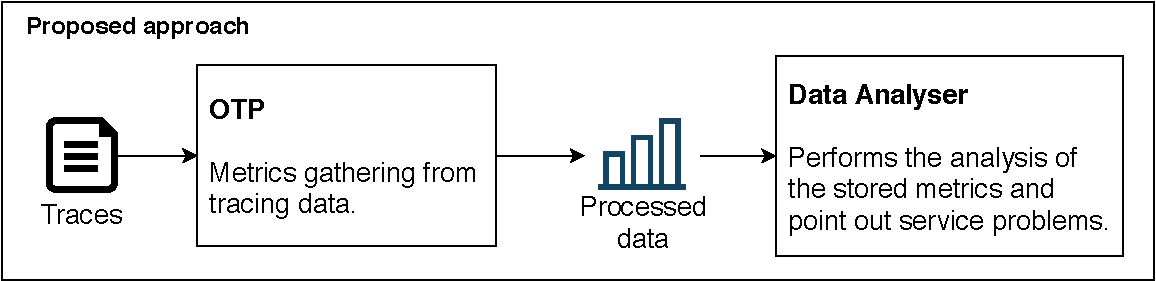
\includegraphics[width=1.00\textwidth]{images/proposed_solution.pdf}
    \caption{Proposed approach.}
    \label{fig:proposed_approach}
\end{figure}

Figure~\ref{fig:proposed_approach} shows the proposed process order for tracing data. We expect to have two main components, one for data extraction and another for data analysis. The input for each are tracing data and processed data from the first component respectively. The outcome is to answer the research questions defined in Section~\ref{sec:research_questions}~-~\nameref{sec:research_questions}.

Next Section~\ref{sec:functional_requirements}~-~\nameref{sec:functional_requirements} covers the functional requirements for this solution.

\section{Functional Requirements}
\label{sec:functional_requirements}

In software engineering, functional requirements defines the intended function of a system and its components. To present the functional requirements for our solution proposition, an id, the corresponding name and its priority are provided. The notation used in priority was based on the urgency that we expected from feature implementation. Three priority levels were used: High, Medium and Low. Therefore, the functional requirements for the proposed solution, sorted by priority levels, are presented in Table~\ref{table:functional_requirements_specification}.

\begin{table}[H]
    \caption{Functional requirements specification.}
    \label{table:functional_requirements_specification}
    \centering
    \begin{tabularx}{\linewidth} {
            |>{\hsize=0.10\hsize}X|
            >{\hsize=0.75\hsize}X|
            >{\hsize=0.15\hsize}X|}
        \cline{1-3}
         \textbf{ID}
         & \textbf{Name}
         & \textbf{Priority}                                                                                                                                                                                  \\ \hline \hline
         FR-1
         & The system must be able to ingest tracing data from a files or external distributed tracing tools.
         & High \\ \hline
         FR-2
         & The system must be able to retrieve service dependency graphs from distributed tracing tools.
         & High \\ \hline
         FR-3
         & The system must be able to store service dependency graphs in a graph database.
         & High \\ \hline
         FR-4
         & The system must be able to store time-series metrics extracted from tracing data in a time-series database.
         & High \\ \hline
         FR-5
         & The system must be able to extract the number of calls per service (total, incoming and outgoing) from tracing data.
         & Medium \\ \hline
         FR-6
         & The system must be able to extract the response time per service from tracing data.
         & Medium \\ \hline
         FR-7
         & The system must be able to generate request work-flow paths from tracing data.
         & Medium \\ \hline
         FR-8
         & The system must be able to calculate request ratio of success and error, for specific services, from tracing data.
         & Medium \\ \hline
         FR-9
         & The system must be able to calculate the degree (total, in and out) of services from service dependency graphs.
         & Medium \\ \hline
         FR-10
         & The system must be able to retrieve the difference between two service dependency graphs.
         & Medium \\ \hline
         FR-11
         & The system must be able to produce a report about spans structure using a defined OpenTracing structural schema.
         & Low \\ \hline
         FR-12
         & The system must be able to calculate the time coverage of traces in a given time-frame.
         & Low \\ \hline
         FR-13
         & The system must be able to identify regions of outliers presented in multiple time-series.
         & Low \\ \hline
    \end{tabularx}
\end{table}

Functional requirements defined in Table~\ref{sec:functional_requirements} were written based on defined research questions presented in Section~\ref{sec:research_questions}. These functional requirements can be grouped in three groups due to their priority levels. The first four (FR-1 to FR-4) are presented with high level of priority, because they represent the base functionality needed to implement the remaining requirements. The next eight functional requirements (FR-5 to FR-11), are time based metric extraction from tracing. The remaining three (FR-12 to FR-14) are related with trace testing and anomaly detection based in time-series thus the low priority.

Next Section~\ref{sec:quality_attributes}~-~\nameref{sec:quality_attributes} covers the proposed approach non-functional requirements.

\section{Quality Attributes}
\label{sec:quality_attributes}

Another important consideration, when designing a software system, is to specify all the quality attributes (also called non-functional requirements). These type of requirements are usually Architecturally Significant Requirements and are the ones that require more from software architect's attention, as they reflect directly all architecture decisions. To specify them, a representation called utility tree is often used. In this tree, the \gls{qa} are placed by an order of priority considering their impact for the architecture and for the business. The priority codification for the \gls{qa} is:
%  in order to consider the trade-offs and decide the weight of each in the produced architecture.

\begin{itemize}
    \item H. High
    \item M. Medium
    \item L. Low
\end{itemize}

To describe them properly, six important aspects must be included in \gls{qa} definition: \emph{stimulus source}, \emph{stimulus}, \emph{environment}, \emph{artefact}, \emph{response} and \emph{measure of the response}.

Figure~\ref{fig:utility_tree} contains all raised \gls{qa} for this proposed solution exposed in an utility tree structure, sorted alphabetically by their general \gls{qa} name, and after by the architectural impact pair (Architecture and Business).

\begin{figure}[H]
    \centering
    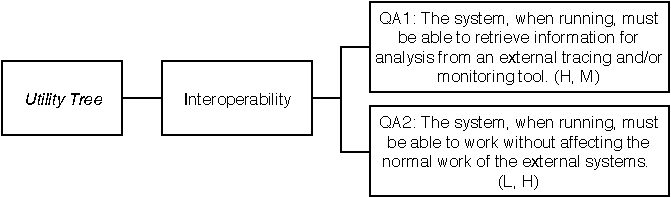
\includegraphics[width=1.00\textwidth]{images/utility_tree.pdf}
    \caption{\gls{qa} utility tree.}
    \label{fig:utility_tree}
\end{figure}

Figure~\ref{fig:utility_tree} shows us that only two Interoperability \gls{qa} were defined. An explanation for both is provided bellow:

\begin{itemize}
    \item[\textbf{QA1}] (Interoperability): Since the proposed solution must ingest tracing data. This information is usually found in distributed tracing tools already used by operators. To gather this information, access to an external distributed tracing tool is an important feature.As this is considered the starting point to obtain our data, we considered a Medium level for the architecture and a Low for the business.

    \item[\textbf{QA2}] (Interoperability): Since the proposed solution will be accessing an external distributed tracing system or outputs generated by it, all interactions with these systems must not cause conflicts. This is very important in the business perspective, because if our solution is not co-habitable with already used systems, it may be completely rejected. For the architectural perspective it does not represent a big impact, and therefore a Low level was assigned.

    %\item[\textbf{QA3}] (Performance): We defined this \gls{qa} taking into account the number of spans produced in an hour, by the system were we gathered our data. As it produces approximately 200.000 spans in an hour, and to ease our research work when using the tool, we decided to set the target for our solution as 1.000.000 spans in about a minute. This \gls{qa} will have an high architectural impact, as it can define a certain technology for graph processing. For the business perspective, we considered a Medium level, as it presents some interest.

    %\item[\textbf{QA4}] (Scalability): Due to the amount of data needed to process and store over time, our system has to be able to store the data into multiple machines because it may start running out of space. We decided to give a medium level of architectural impact as it can change the solution in terms of storage components. For the business this has an high impact, as it need more machines to run the solution if this \gls{qa} is fully considered against the remaining.

    %\item[\textbf{QA5}] (Traceability): This \gls{qa} was considered due to the simple fact that we need to bee able to see what's the system is doing, when it's processing the data. For this \gls{qa} we decided to give low levels for both architecture and business, as it does not represent relevance to any of them.

    %\item[\textbf{QA6}] (Testability): As the system will be analysing external systems, we need to be sure that it analyses it in a correct way, and to be sure of this we need to test our solution. We considered a medium level for the architectural impact for this \gls{qa}, because its implementation needs to analyse some components from within the system. For the business we considered a low level, because the main interest to test the system is ours in order check if it is working correctly.
\end{itemize}

\section{Technical Restrictions}
\label{sec:technical_restrictions}

In this Section, technical restrictions considered in proposed solution are presented.

In software engineering, after specifying functional and non-functional requirements for a solution, comes the specification of business restrictions, however, in this project none were raised due to the fact that this work is focused on exploration and research.
%, and that there isn't any formal client defined.

To define the technical restrictions, we used an id and its corresponding description. Table~\ref{table:technical_restrictions_specification} presents the technical restrictions considered for the proposed solution.

\begin{table}[H]
    \caption{Technical restrictions specification.}
    \label{table:technical_restrictions_specification}
    \centering
    \begin{tabularx}{\linewidth} {
        |>{\hsize=0.25\hsize}X|
        >{\hsize=0.75\hsize}X| }
        \cline{1-2}
        \textbf{ID}
         & \textbf{Description}                    \\ \hline
        TR-1
         & Use \emph{OpenTSDB} as a Time-Series database. \\ \hline
    \end{tabularx}
\end{table}

Table~\ref{table:technical_restrictions_specification} shows that we have raised only one technical restriction. This technical restriction was considered because Professor Jorge Cardoso, acting as a client for this solution demanded it. \emph{OpenTSDB} is the database that they are currently using in their projects at Huawei Research Center. This restriction will ease their work to introduce changes if needed.
%However, this project does not have a concrete and formally defined client, it is good to use a technology used by the people that will use the tool to ease their work and possibly introduce changes.

\section{Architecture}
\label{sec:architecture}

In this Section, the architecture is presented based on all previous topics with resource to the defined Simon Brown’s C4 Model~\cite{simon_browns_c4_model}. This approach of defining an architecture uses four diagrams: \emph{1 - Context Diagram}, \emph{2 - Container Diagram}, \emph{3 - Component Diagram} and \emph{4 - Code Diagram}. To define the architecture for our solution, only the first three representations were considered. Every representation will be exposed with a explanation of the decisions taken to draw each diagram. After presenting the representations and the corresponding explanations, we will cycle thought all architectural drivers: \gls{qa}, bussines and technical restrictions, in order to explain where they are reflected and the considerations taken to produce this architecture.

\subsection{Context Diagram}
\label{subsec:context_diagram}

In this Subsection the context diagram is presented. This diagram allows us to see ``the big picture'' of the overall system as it represents the system as a ``big box'' and the corresponding interactions with users and external software systems. Figure~\ref{fig:context_diagram} presents the context diagram for this solution.

\begin{figure}[H]
    \centering
    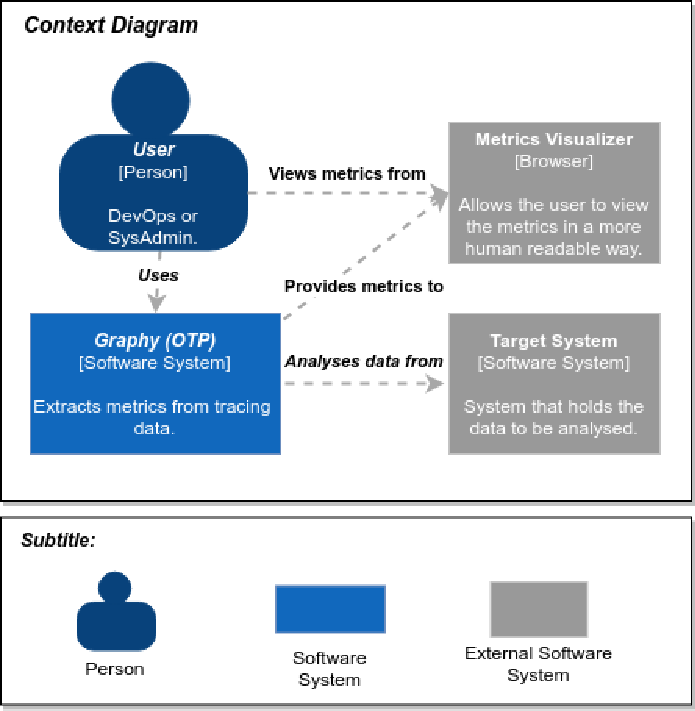
\includegraphics[width=1.0\textwidth]{images/context_diagram.pdf}
    \caption{Context diagram.}
    \label{fig:context_diagram}
\end{figure}

From Figure~\ref{fig:context_diagram}, we can see that our solution, named \emph{Graphy \gls{otp}}, receives interactions from users, as it need someone to start the whole process. This piece of software analyses data from an external target system that holds the tracing information and consequently, provides extracted metrics to an external metrics visualizer component. Users can view extracted metrics from this last component. Also, reports are produced and stored within our solution, when it performs tracing analysis. 

\subsection{Container Diagram}
\label{subsec:container_diagram}

The container diagram is presented in this Subsection. This type of diagram allows us to ``zoom-in'' in the context diagram, and get a new overview of our solution. Therefore, in this diagram we are able to see a high-level shape of the software architecture and how responsibilities are distributed across containers. Figure~\ref{fig:container_diagram} presents the container diagram for our proposed solution.

\begin{figure}[H]
    \centering
    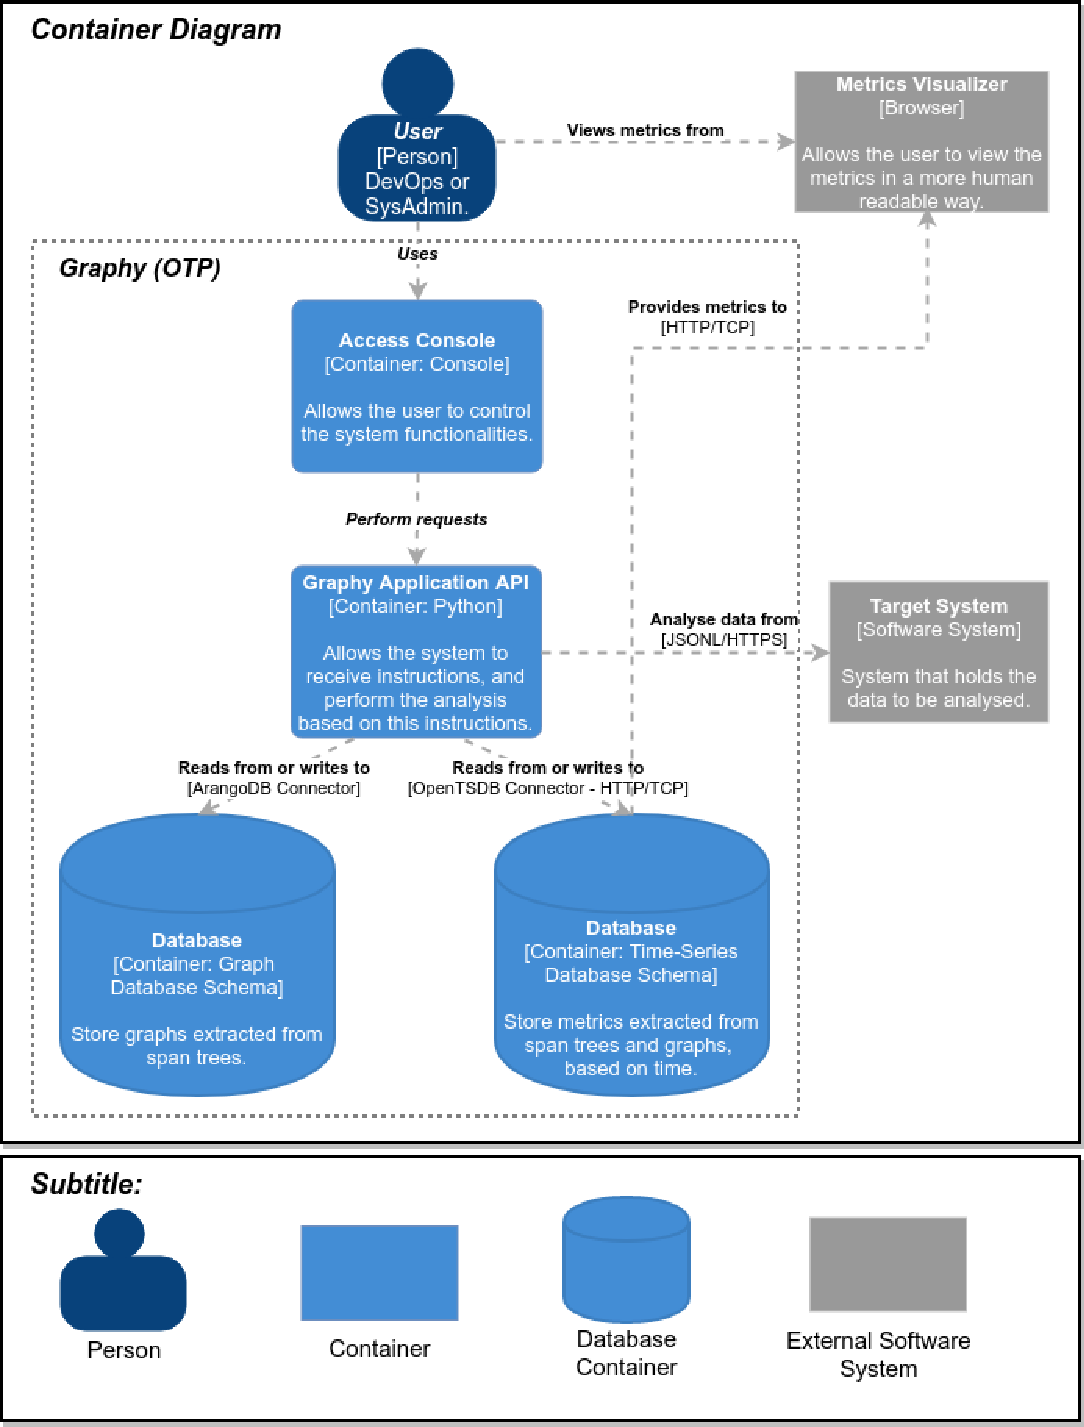
\includegraphics[width=1.00\textwidth]{images/container_diagram.pdf}
    \caption{Container diagram.}
    \label{fig:container_diagram}
\end{figure}

\newpage

Figure~\ref{fig:container_diagram} contains the main containers involved in our solution. The first one, from top to bottom, is the \emph{Access Console} and this container was considered as it is needed for the user to be able interact with the \emph{Graphy \gls{api}}. This last one controls the entire OpenTracing system, uses a communication protocol to retrieve tracing information from external target system, and two databases to store the information resulted from processing tracing data -- a \gls{gdb} and a \gls{tsdb}. The second database provides metrics to be visualized in an external metrics visualizer system.

\subsection{Component Diagram}
\label{subsec:component_diagram}

This Subsection contains the last diagram, the component diagram. This type of diagram gives a more deeper vision about the system, and therefore, it reveals the main components. Figure~\ref{fig:component_diagram} presents the component diagram for this solution.

\begin{figure}[]
    \centering
    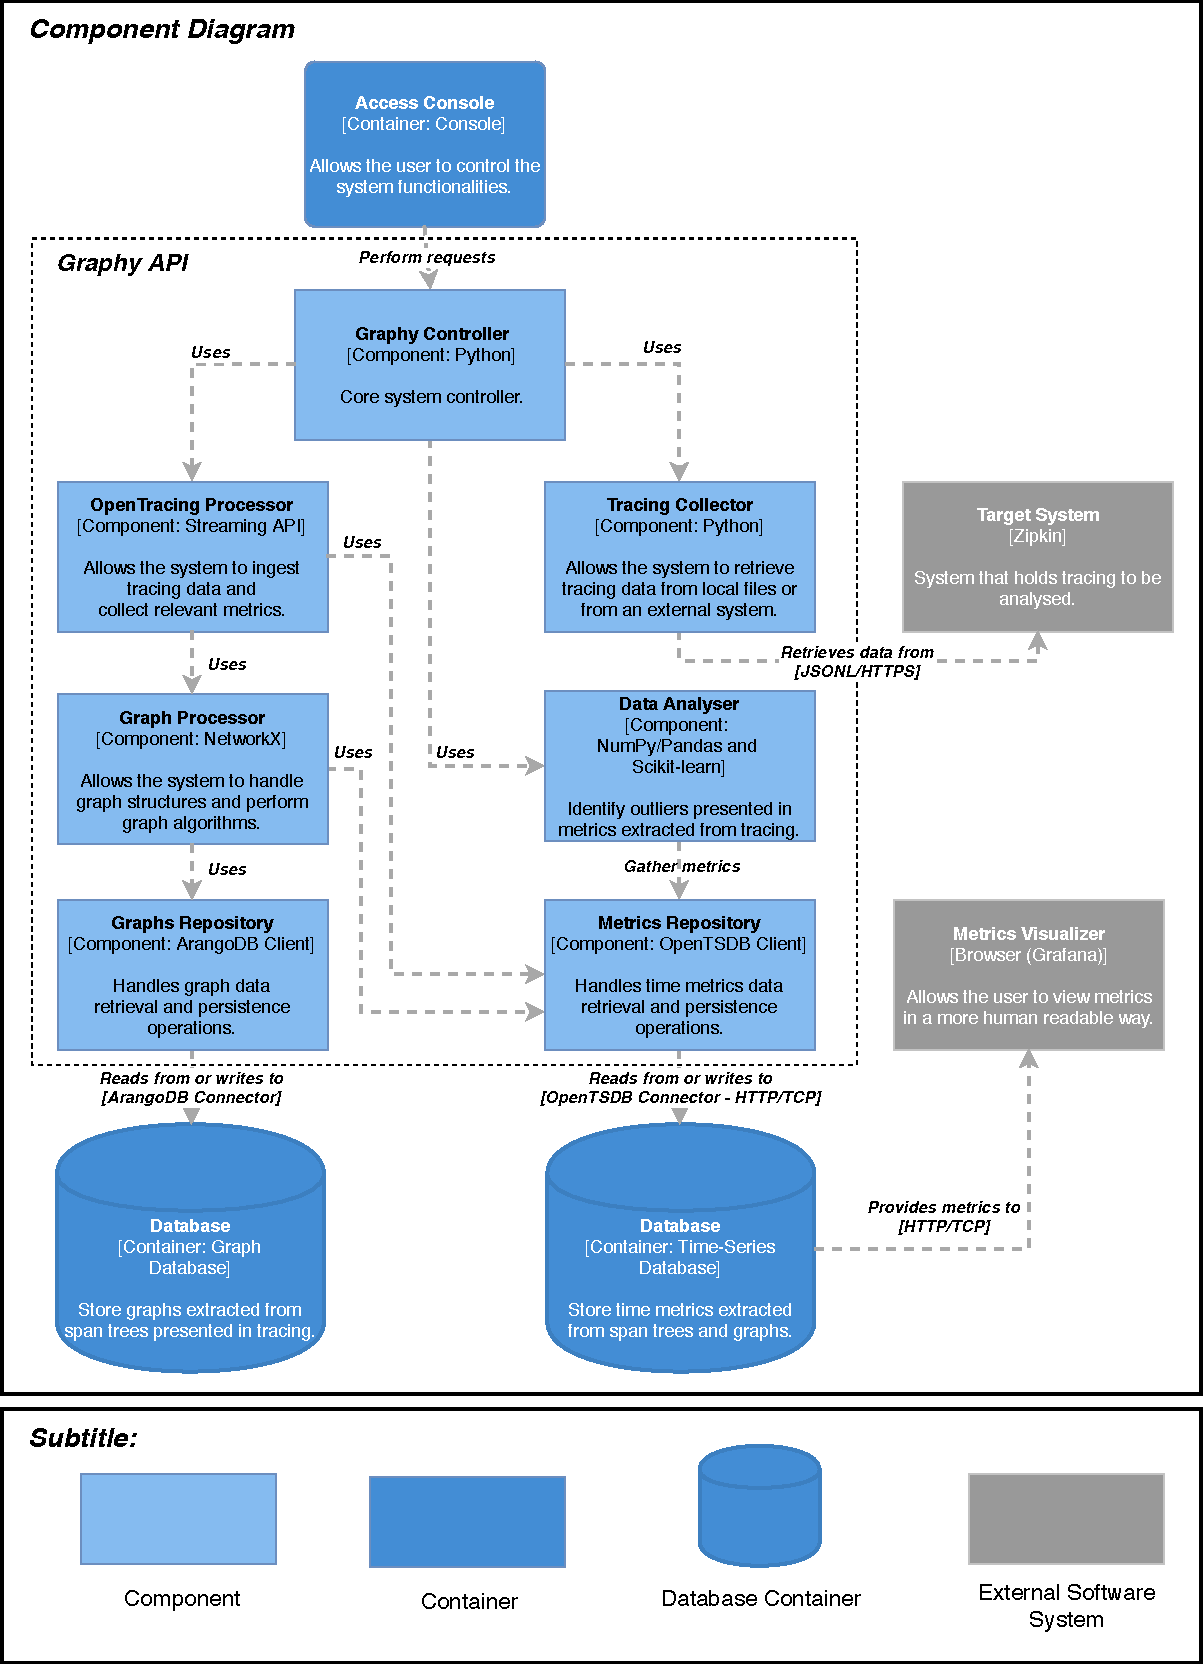
\includegraphics[width=1.00\textwidth]{images/component_diagram.pdf}
    \caption{Component diagram.}
    \label{fig:component_diagram}
\end{figure}

Figure~\ref{fig:component_diagram} provides us with a lower level visualization of \emph{Graphy API} container composed by eight components. At its core we have \emph{Graphy Controller}, a component with the responsibility of receiving requests from the user through \emph{Access Console} and control \emph{OpenTracing Processor}, \emph{Tracing Collector} and \emph{Data Analyser} components. The first one has the objective of mapping tracing data, span trees and service dependency graphs instantiation into memory. The second one collects tracing, the information that feeds this entire application, from local files or from external systems, e.g., \emph{Zipkin}. The last one, \emph{Data Analyser}, identifies outliers presented in time-series metrics extracted from tracing, allowing our solution to detect anomalous services presented in distributed systems. \emph{Graph Processor} is the component for graphs handling, thus it has the capability of performing operations over graphs, e.g., subtract one graph from another, extract node degrees and count connections between nodes. The remaining components, \emph{Graphs Repository} and \emph{Metrics Repository}, are used to map graphs and time-series metrics, respectively, into and from their corresponding databases.

To check the architecture produced, we will now cycle between both \gls{qa} and check were they are reflected in the architecture presented for this solution, explaining the trade-off involved and what were our considerations about each one.

\gls{qa}1 and \gls{qa}2 are satisfied by the fact that the system is able to collect data from an external system. Using a communication protocol where data is exchanged thought \gls{http} and exposed \gls{api}, allows to externally request little chucks of data from target systems without interfering with their normal function.

%\gls{qa}3 is satisfied when we decide to use NetworkX as the technology to process our graphs. This technology does not scale horizontally, however it has a very decent performance and it's able to retrieve a certain measure of a graph with about 100.000 nodes, in near 15 seconds\cite{networkx_speed}. From 1.000.000 spans, in normal conditions, we will never be able to get a graph of this kind of size, as with our experiments, with 100.000 spans we were able to get a graph of almost 20 nodes, and with 200.000 spans we were able to get a graph of almost 30 nodes. In the end, we are considering this time and span quantity to be sure that our tool will give us good times and ease our work of performing the research and implementation of this kind of tool.

%\gls{qa}4 is satisfied because we decided to use two databases that are scalable horizontally by design, the ArangoDb for a \gls{gdb} and the \emph{OpenTSDB} for a \gls{tsdb}, both presented in the \ref{subsec:graph_database_tools} and \ref{subsec:time_series_database_tools} subsections respectively. In the end, this \gls{qa} can not be fully satisfied because we can not scale our system entirely, due to the fact of the technology that we chose to perform the graph processing. However, we have chosen this technology because it can perform much more graph algorithms, as we can see in the figure \ref{fig:graph_manipulation_and_performance_tools_diagram_comparison}, and this is much more relevant for our main purpose.

%\gls{qa}5 is satisfied by the existence of the component \textit{Logging Component}, that allows the system to perform logging of relevant information. For the technology here, we decided to use click-log\cite{click_log_doc}, a python library used for logging purposes as it has all the main capabilities needed here to perform the logging.

%\gls{qa}6, like the previous one is satisfied by the existence of a certain component, the \textit{Testing Component}, which implements all the capabilities and functionalities to perform tests and check if the systems is working correctly.

Finally, for the only technical restriction raised, we can see that it is satisfied by the usage of \emph{OpenTSDB} as the main \gls{tsdb} for our solution.

This solution does not have many architectural drivers: quality attributes, business constraints and technical restrictions, due to being a prototype. The main objective is to produce a solution capable of explore tracing data allowing us to conduct a research about what we can do with tracing, therefore it does not have many architectural constraints. Nevertheless, with the presentation of these four sections, we conclude that our solution satisfies all the architectural drivers, and therefore, we may claim that the proposed architecture fits our needs as a solution.

Next Chapter,~\ref{chap:implementation_process}~-~\nameref{chap:implementation_process}, covers the implementation of the solution presented in the current chapter. All implemented algorithms and technical decisions are discussed and explained in detail.

\checkoddpage
\ifthenelse{\boolean{oddpage}}
{ % Odd page
    \newpage
    \blankpage}
{ % Even page
}
\glsresetall
% Implementation Process -------------------------------------------------------------------------
\chapter{Implementation Process}
\label{chap:implementation_process}

This chapter presents the implementation process of the proposed solution explained in the previous chapter. Every step is explained taking into consideration the most important points to implement the methods. This chapter covers three main sections: First, \ref{sec:data_set} - \nameref{sec:data_set}, the data provided to perform this research is briefly exposed and analysed. Second, \ref{sec:metrics_gathering} - \nameref{sec:metrics_gathering}, the implementation of Graphy (\gls{otp}), our proposed solution to collect metrics from tracing data presented in the chapter \ref{chap:possible_solution}, is explained in detail. Finally, \ref{sec:observations_analysis} - \nameref{sec:observations_analysis}, the methods for analysis of the stored observations are presented with the respective results and answers to the research questions.

\section{Huawei Tracing Data Set}
\label{sec:huawei_tracing_data_set}

Nothing comes from nothing, and in this project the starting point for every method developed was a data set provided by Huawei, represented by professor Jorge Cardoso. To be able to get access to this information, a NDA: Non-disclosure agreement were signed by both parts. This data set contains the results of tracing data gathered from an experimental cluster used by the company for testing purposes. In terms of time this data is a representation of two days of the systems workload, therefore two files were provided, one for each day. These files were generated in 2018-07-10 and for protection, some fields of the data set were obfuscated during the generation process.

\begin{table}[H]
\caption{Data set provided for this research.}
\label{table:data_set_provided_for_this_research}
\centering
\large
\begin{tabularx}{\linewidth} {
    |>{\hsize=0.70\hsize}X| 
     >{\hsize=1.15\hsize}X|
     >{\hsize=1.15\hsize}X| }
     \hline
    
    & 2018-06-28
    & 2018-06-29 \\ \hline
    \textbf{File}
    & traces-2018-06-28.jsonl
    & traces-2018-06-29.jsonl \\ \hline
    % \textbf{Size}
    % & 130 megabytes
    % & 164 megabytes \\ \hline
    \textbf{Spans count}
    & 190 202
    & 239 693 \\ \hline
    \textbf{Traces count}
    & 64 394
    & 74 331 \\ \hline
\end{tabularx}
\end{table}

As we can see by the information presented in the table \ref{table:data_set_provided_for_this_research}, each file represents a day of traces and both were written in JSONL format \cite{jsonl}. This type of file format is an extension to the normal lightweight data-interchange standard JSON: JavaScript Object Notation file type, however, in JSONL multiple JSONs are separated by a new line character. Each Span is presented by a single JSON, so for each line we have a Span encoded in JSON format. Further in this sections is a representations of the amount of traces by hour, to do this and to perform the traces count we have to map the span trees, the explanation and algorithm are presented in the next section \ref{sec:metrics_gathering} - \nameref{sec:metrics_gathering}.

Span data format is defined in a specification, but companies and software developers do not need to strictly follow it, they can produce their own span data format and this means that each software company can have their own span specification. To ensure the understanding and follow up with the span data format, there was a file with instructions about the spans. In this file, the fields were explained, this consisted in their specific names and the supposed data type. A brief sample of the explanation provided in the file is exposed in the points bellow.

\begin{enumerate}[topsep=1pt, partopsep=1pt, itemsep=5pt, parsep=5pt]
    \item traceId - Unique id of a trace (128-bit string).
    \item name - Human-readable title of the instrumented function.
    \item timestamp - UNIX epoch in milliseconds.
    \item id - Unique id of the span (64-bit string).
    \item parentId - Reference to id of parent span.
    \item duration - Span duration in microseconds.
    \item binaryAnnotations:
    \begin{enumerate}[topsep=1pt, partopsep=1pt, itemsep=5pt, parsep=5pt]
        \item protocol - 'HTTP' or 'function' for RPC calls.
        \item http.url - HTTP endpoint.
        \item http.status\textunderscore code - Result of the HTTP operation. 
    \end{enumerate}
    \item annotations:
    \begin{enumerate}[topsep=1pt, partopsep=1pt, itemsep=5pt, parsep=5pt]
        \item value - Describes the position in trace (based on Zipkin format). Could be one of the following values or other: 'cs' (client send), 'cr' (client receive), 'ss' (server send) or 'sr' (server receive)
        \item timestamp - UNIX epoch in microseconds.
        \item endpoint - Wich endpoint generated a trace event.
    \end{enumerate}
\end{enumerate}

Two notes were also provided within this file. To point each one, has they are very important, we present them bellow.

\begin{enumerate}[topsep=1pt, partopsep=1pt, itemsep=5pt, parsep=5pt]
    \item Time units are not consistent, some fields are in milliseconds and some are in microseconds.
    \item Trace spans may contain more fields, except those mentioned here.
\end{enumerate}

From the point presented above, we get a notion that we need to consider some things about the values that we might encounter in the spans fields. Some fields are required by the OpenTracing specification as presented in \ref{subsec:distributed_tracing}, and to sanitise this whole topic, it is very important that a company, when producing this kind of information, stick with the specification, even if it is an open-source specification. So "traceId", "name", "timestamp", "id" and "parentId" are required fields, this is because they are the foundations to identify a span, produce relation between them and to place them in time. Other topic that is very important to understand is that the specification is not precise, we do not know clearly what is available when working with a span, this means that there is no specific data structure for fields like "binaryAnnotations" and "annotations", and this is a big problem as we might have spans that are completed or incomplete and we can not know it as there is nothing to tell us about it. For example, in the "binaryAnnotations" the information is disposed in key value objects, and as said in the second point of the notes presented above: "Trace spans may contain more fields, except those mentioned here", this causes a tremendous explosion in possibilities, because there might be keys with their corresponding values for some particular spans and it gets hard to generalise this whole span structure.

At the current time of writing, the clarity of span data only depends if the company that produced the software or the software owner care about what the system will produce in terms of tracing data. To be sure that the teams developing distributed software produce good tracing data, the company must implement a standard for every team to follow. The normalisation and unification of the span format should be one thing to consider in the near future, this is because it is very hard to perceive and distinguish multiple span types. For example, in the data provided spans can be of two types: \gls{http} Span or \gls{rpc} Span, and the only field that distinguishes them is that the second one has an "exec" field, which stands for the execution process id, and that is not presented in the HTTP span type. Another example, for the measure units of some fields, if the field have the same key, they all should be in one single measure unit, this is because some tools are expecting this, and they assume wrong values when spans have time-stamps in milliseconds and others in microseconds like in this case.

To give a brief notion of how the traces and spans are spread throughout time, we have used our tool, \todo{Graphy \gls{otp}}, to generate two charts that represents the counting of traces and spans for each hour in each day. The decision to generate two spitted charts comes from the simple fact that we have one file for each day. To be able to count the spans in time, in this case by hour, the tool only needs to group every span by hour and count them, however for traces, the tool has a lot more work has it have to merge all spans in their corresponding trace (explained in \ref{sec:metrics_gathering}. After having all traces, we can count them like we count spans. Note that if a span or trace starts at a given time (t1) contained in a time-frame (tf1), and with its duration (d1) surpasses the next time-frame (tf2), (t1 + d1 \textgreater tf2), it is considered to be in the tf1, or by other words, only the starting time of the trace or span is considered for the counting. The figures \ref{fig:trace_file_count_2018_06_28} and \ref{fig:trace_file_count_2018_06_29} presents the data set traces and spans counting throughout time.

\begin{figure}[H]
    \centering
    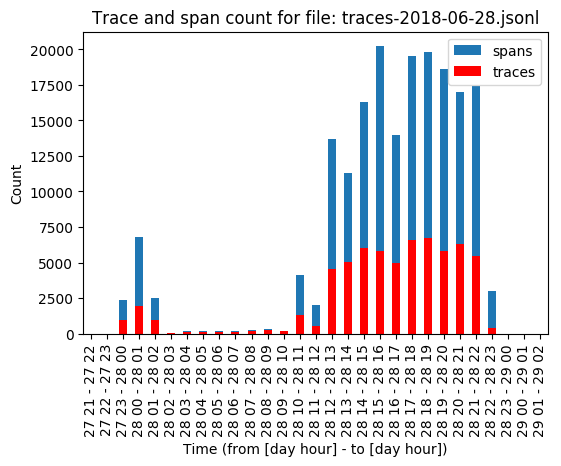
\includegraphics[width=0.88\textwidth]{images/trace_file_count_2018_06_28_chart.png}
    \caption{Trace file count for 2018-06-28.}
    \label{fig:trace_file_count_2018_06_28}
\end{figure}

\begin{figure}[H]
    \centering
    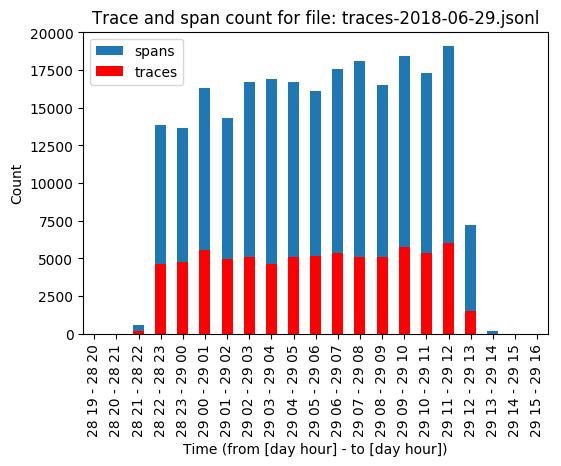
\includegraphics[width=0.88\textwidth]{images/trace_file_count_2018_06_29_chart.png}
    \caption{Trace file count for 2018-06-29.}
    \label{fig:trace_file_count_2018_06_29}
\end{figure}

// A big region without traces, why? Can't answer that!

// Less data spreaded through time than the previous one.

// Maybe include here the Quality of tracing analysis and possibilities in their own analysis.


\section{Open Tracing Processor Component}
\label{sec:open_tracing_processor_component}

Start by explaining how the metrics relate with the questions, and what metrics we decided to extract and were, how do we put it there.

Explain how to map spans into span trees.
to process the information presented in the data set and store it for our own analysis purposes

... as explained in \ref{subsec:traces_and_spans}, each spans relates with another, in this case, by a field called parent id. After mapping the spans into trees, we end up with a list of tress, each for a specific trace, and we just have to count them. To map the spans into trees, we index it by the 

// TODO: Regarding database setup and implementations, the choices were to use OpenTSDB as a Time-Series database and ArangoDB as a graph database. However, the second choice wasn't the better one, due to some lack of support and terrible \gls{api} documentation. Some issues were opened in the GitHub client \gls{api} for the programming language Python, but the answer was always that it have the expected behaviour \cite{arango_issues}. This have lead to some difficulties when implementing the component Graphs Repository, presented in Graphy API. Some difficulties were felted when trying to store graphs with custom names and setting up different type values to some data structures presented in the pyArango client API. The solution was to fetch all the API, perform some changes and use our custom pyArango client. This changes were committed for review to the original project stored on GitHub. Mitigating this kind of problems was something that was impossible to predict when choosing the Graph storing technology.

\begin{algorithm}[H]
\SetAlgoLined
\KwResult{Write here the result }
 initialization\;
 \While{While condition}{
  instructions\;
  \eIf{condition}{
   instructions1\;
   instructions2\;
   }{
   instructions3\;
  }
 }
 \caption{How to write algorithms}
\end{algorithm}

\todo{aaa}

// Finally present the display of information in the Grafana with some prints. Refer that the lack of data in day 28. And do some observations. 

% Observations Analysis --------------------------------------------------------------------------
\section{Data Analysis Component}
\label{sec:data_analysis_component}

// TODO: Talk about Unlabeled data, the best algorithms to handle this kind of situation and how we did it.


%-------------------------------------------------------------------------------------------------


%-------------------------------------------------------------------------------------------------
\checkoddpage
\ifthenelse{\boolean{oddpage}}
{ % Odd page
\newpage
\blankpage}
{ % Even page
}
%-------------------------------------------------------------------------------------------------
\glsresetall
\chapter{Results, Analysis and Limitations}
\label{chap:results_analysis_and_limitations}

\todo{Section intro...}

\section{Anomaly Detection}
\label{sec:anomaly_detection}

\todo{...}

\section{Trace Quality Analysis}
\label{sec:trace_quality_analysis}

\todo{...}

%\section{Results Analysis}
%\label{sec:results_analysis}
%
%\todo{...}

\section{Limitations of OpenTracing Data}
\label{sec:limitations_of_opentracing_data}

\todo{...}

%-------------------------------------------------------------------------------------------------
\checkoddpage
\ifthenelse{\boolean{oddpage}}
{ % Odd page
\newpage
\blankpage}
{ % Even page
}
%-------------------------------------------------------------------------------------------------
\glsresetall
\chapter{Conclusion and Future Work}
\label{chap:conclusion_and_future_work}

This chapter presents the conclusion and the future directions of work that can follow this research project. Therefore, this chapter contains a summary about what was done, the main conclusions and contributions, followed by a brief reflection about the achievements of this research and the future work that can follow from these achievements.

% FROM PAPER
%This Section covers three main topics. It contains a summary about what was done and what were the main conclusions extracted from this research followed by brief reflections regarding this whole research topic and ending with the future work and research path that we hope to be taken in the future.

%\subsection{Summary}
%\label{subsec:summary}

After this whole research, we are able to state that tracing data is useful and required to find anomalies related to service morphology. However, this type of data is hard to handle and one must use it if some issue was detected in metrics easier to analyse, e.g. monitoring. For this type of data to be easier to analyse, a discussion is provided about this difficulty bellow. So, in the end our perception is that, there are issues that we can only perceive using tracing data, but it is very expensive to analyse this data directly.

Regarding the remaining topic, the analysis of tracing, both tests are very interesting but, due to lack of required and strict specification, the tests and results of the ``structural quality analysis'' using spans are not very useful however, one can state that this is all we can do taking into consideration the OpenTracing specification.

%\subsection{Brief reflections}
%\label{subsec:brief_reflections}

In the end, our analysis of the provided tracing data generated by Huawei cluster, took us to the following conclusions about \emph{OpenTracing}:

\begin{enumerate}
    \item \emph{OpenTracing} suffers from a lack of tools for data processing and visualisation.
    \item The \emph{OpenTracing} specification is ambiguous.
    \item The lack of tools to control instrumentation quality jeopardizes the tracing effort.

    \item Lack of tools for OpenTracing processing and visualisation.
    \item Ambiguity presented in the OpenTracing specification.
\end{enumerate}

One point to consider is that it was difficult to find tools for tracing data visualisation and processing. Only Zipkin and Jaeger, presented in the Subsection~\ref{subsec:distributed_tracing_tools}, represent some usefulness has they allow distributed tracing visualisation in a more human readable way. However, they do not present any kind of tracing analysis. So, because of this, there are real needs for tools that can handle this kind of data.

The second point is the big problem with the OpenTracing specification. The main difficulties in implementing the tools mentioned in this paper were felt because of the ambiguity in tracing data. The specification allows many fields that are not strictly defined. As mentioned in Section~\ref{sec:second_question}, one of the detected problems are in the measurement units. Other problem resides in some fields that contain very important information about the path of the request, these fields are defined as maps of key - values, where the keys can be anything that the programmer wants. This brings a big problem, because tools must perceive this kind of values and some of them may not be considered for analysis. A simple solution could be to redefine the specification and reduce these kind of fields, transforming the specification into a more strict schema. This would allow the implementation of more general trace processing tools.

%\subsection{Future work}
%\label{subsec:future_work}

Therefore, from the worked developed in this thesis, we have some considerations and        
From this work there are some paths to consider for future work:

\begin{enumerate}
    \item Improve and develop new tools for OpenTracing processing.
    \item Perform a research to redefine the OpenTracing specification. 
    \item Explore and analyse the remaining extracted tracing metrics.
    \item Use tracing data from other systems.
    \item Develop a simulated system with the capability of fault-injection to prove the analysis observations.
    \item Conciliate the results from tracing data with other kinds of data like monitoring and logging.
    \item Follow closely the development and the community of \emph{OpenTelemetry} project, and contribute with ideas generated by this research.
\end{enumerate}

First, today there are not many tools for processing and handling OpenTracing data. This increased difficulty because when we needed to process this kind of data in a different way, we always ended up developing everything from scratch.

Second, there must be a way to eliminate or reduce the ambiguity and uncertainty of data presented in tracing generated by non-strict fields. If the specification can not be changed, a new way to transform tracing data to ease the analysis is very welcome.

Third, these developed tools extract many more metrics. The majority of them were not explored due to lack of time, and therefore, here resides the opportunity to do it. The path starts by defining new research questions that use these metrics and develop ways to analyse them.

Fourth, just one data set of tracing data was used in this research. Test the tools and methods with other tracing data could be interesting.

Fifth, the system were the data was gathered was a company testing system. One good future approach was to have a microservice based simulated system, were the developers could inject faults like request flow redirection, latency issues, and others, point them out and test the developed tools and methods.

Sixth, only tracing data was used in this research, one interesting path to follow is to have more kinds of data like monitoring and logging from the target system. This could help the analysis of the system, due to more knowing about it.

\todo{Add a final paragraph saying that this whole work was a succes due to the technologies that were developed, the answers provided to research questions and the resulting paper for the IEEE NCA.}

%\section{Brief Reflection}
%\label{sec:brief_reflection}
%
%\todo{This thesis presents an attempt to further the field of distributed system %based tracing analysis.}
%
%\todo{...}
%
%\todo{A reflection about the tools and methods produced and the open paths from %this whole research are exposed. Also a reflection of the main difficulties %felted with this research are presented}
%
%\section{Future Work}
%\label{sec:future_work}
%
%\todo{Talk a bit about the possible work in this field and what can be achieved %using this work.}
%
%\todo{the future work that can be addressed considering this work is properly %explained taking into consideration what is said in the previous section}
%
%\section{Concluding Research Questions}
%\label{sec:concluding_research_questions}
%
%\todo{...}
%
%\todo{EXTRACTED FROM PAPER! (KEEP ONLY THIS?)}

\checkoddpage
\ifthenelse{\boolean{oddpage}}
{ % Odd page
\newpage
\blankpage}
{ % Even page
}

\printbibliography[title={References}]
\newpage

% TODO: Uncomment the following for the final report delivery
%\begin{appendices}
%\input{chapters/9-appendices}
%\end{appendices}
%------------------------------

\end{document}